%% RSAA THESIS 'TEMPLATE' BY JOSHUA RICH <joshua.rich@gmail.com>
%% README:
% This template is designed to be used with pdflatex rather than plain
% latex.  It was developed under a TeXLive 2007 TeX distribution on
% Linux.  

% for requirements of typesetting and formatting see:
% http://info.anu.edu.au/Policies/_REG/Guidelines/PhD_Exam_Theses.asp
% (in emacs, type M-x browse-url with the cursor on 
% the link above)

%%NOTES ABOUT THE DOCUMENT CLASS
% Yes, I'm using a report style.  Any 'thesis style' you might
% find or someone will give you is based on the standard report
% class, but is probably well outdated compared to whatever TeX
% you have installed.  Besides, why use that style file if you 
% have no idea what it actually does?  You will probably just redefine
% all of its customisations anyway...
\documentclass[11pt,twoside,openright, pdftex]{report} 

% define some constants that can be used in various places to easily
% specify title, subjects, author etc.
\newcommand{\thesistitle}{Type Ia Supernovae: Explosions and Progenitors}
\newcommand{\fullname}{Wolfgang Eitel Kerzendorf}
\newcommand{\shortname}{W. E. Kerzendorf}
\newcommand{\thesissubjects}{stars: supernovae: progenitors --- stars: binaries: symbiotic ---
stars: supernovae: individual (SN 1572, SN 1006)}

%%NOTES ABOUT BABEL PACKAGE:
% It requires two components; the 
% \usepackage line above and the language put in the \documentclass.
% 'british' is used because that is the english style required for an
% ANU thesis.  This will ensure LaTeX uses british hyphenation and
% other language constructs when generating the text.  Putting the
% babel usepackage at the very top also ensures other packages called
% through \usepackage can take advantage of babel if they are set up
% for such.  
% We can also do tricky things in our ~/.emacs file if we
% are an emacs user now as well.  Grab the flyspell-babel and
% ispell-multi  emacs packages from:
% http://www.dur.ac.uk/p.j.heslin/Software/Emacs/
% And put it somewhere Emacs can find it (probably under ~/.emacs.d).
% Then add the following lines to your .emacs:
%   (dolist (hook '(LaTeX-mode-hook))
%   (add-hook hook (lambda () (flyspell-mode 1))))
%   (add-hook 'tex-mode-hook (function (lambda () (setq ispell-parser 'tex))))
%   (autoload 'flyspell-babel-setup "flyspell-babel")
%   (add-hook 'latex-mode-hook 'flyspell-babel-setup)
% After this, you should have Emacs auto-suggesting word corrections
% AND doing it in british-english automagically.  You can do a similar trick
% for papers by simply changing 'british' above to 'american', and
% flyspell will check your paper in american-english.
\usepackage[british]{babel}

%\usepackage{hyperref}

% ---------------------------------------------------------------------
% page size and margins
% ---------------------------------------------------------------------
%%NOTES ABOUT GEOMETRY PACKAGE:
% Below is using the geometry package as it is just cool.  This allows
% you to directly specify the margin requirements as outlined by ANU
% directly.  Here the inner border is 4cm and the outer is 2cm.  Top
% and bottom are also 2cm.  This is much easier than trying to work
% out page and margin dimensions by hand.  This is how you should use
% LaTeX...
\usepackage{geometry}
\geometry{a4paper,twoside}
\geometry{includehead,includefoot}
\geometry{hmargin={4cm,2cm}}
\geometry{vmargin={2cm,2cm}}

% ---------------------------------------------------------------------
% miscellaneous packages used
% ---------------------------------------------------------------------
\usepackage[hiresbb]{graphicx}
\DeclareGraphicsExtensions{.pdf}
%\DeclareGraphicsExtensions{.eps}
\usepackage[twoside]{rotating}

%%NOTES ABOUT FONTS PACKAGES:
% The basic requirements for fonts in an ANU thesis demand clear
% readability and that is about all.  So if you choose a nice,
% standard serif font you won't have any problems.
% I several font families in my thesis below:
%  pxfonts: math typesetting
%  tgpagella: for the normal text font (serif)
%  tgheros: for the sans serif font
%  tgcursor: for the typewriter style font
% TeX Gyre Pagella, Heros and Cursor are part of the TeX Gyre family
% of fonts, which can be obtained from:
%   http://www.gust.org.pl/projects/e-foundry/tex-gyre/
% Not all of the TeX Gyre, and possibly not the latest glyphs are
% available in standard TeX distributions.  
%
% The 'mathpazo' package provides an almost identical, albeit not
% actively developed font family to TeX Gyre Pagella and is included
% in standard TeX distributions.  This package
% also provides a full range of math glyphs.  You'd need to find
% alternative sans serif and typewriter fonts to use with this package.
%
% You can see a whole heap of LaTeX fonts, most of which are also in a
% standard TeX distribution at: 
%  http://www.tug.dk/FontCatalogue/
% This web-page shows what each font looks like and what you need to
% do to include the font in your document.  Note it lists fonts that
% may not be installed by your default TeX installation...
%
% Another list of fonts, recommended by `typophiles' can be found at:
%  http://typophile.com/node/18207
% Although the above list includes some really nice fonts, their
% availability in TeX distributions varies.  You may have to install
% them manually...
\usepackage{xfrac}
\usepackage[T1]{fontenc}
\usepackage{textcomp}
\usepackage{ucs}
\usepackage[utf8x]{inputenc}
\usepackage{amsmath,amssymb}
\usepackage{pxfonts}
\usepackage{tgheros,tgpagella}
\renewcommand*\ttdefault{qcr}
\linespread{1.05} % tgpagella/mathpazo need a bigger line spacing
\usepackage{microtype}
% bibliography uses natbib, this will be a requirement
\usepackage[round]{natbib}
% Super-nice looking tables, better than deluxetable
\usepackage{ctable, longtable}
%%NOTES ABOUT CAPTION AND SUBFIG PACKAGES
% I'm using the caption package to style my captions.
% You need to read the documentation for this package (on CTAN) as it
% has simple explanations of the options and examples of what it looks
% like.
%
% The subfig package allows the ability to control in detail
% positioning of sub-plots in a complex figure as well as add labels
% to them, which can then be referenced in the text without the need
% for changing the actual number as your sub-figures change.
% The subfig package inherits options from the caption package, so
% declare them together.
%
\usepackage[l2tabu, orthodox]{nag}
\usepackage[]{caption,subfig}
\usepackage{captcont}
\captionsetup{format=hang,%
%  indention=-1.5cm,%
  labelsep=quad,%
  labelfont={footnotesize,bf},%
  textfont={footnotesize}}
% The hyperref package is a must while editing.  It provides urls
% inside your document; you can then click to go to certain pages,
% figures or bibliography entries.
\usepackage[pdftex,hyperindex, unicode,pageanchor,plainpages=false]{hyperref}
% \hypersetup{pdftitle=\thesistitle\ - \shortname,%
%   pdfauthor=\fullname,%
%   pdfsubject={\thesissubjects},%
%   citecolor=DodgerBlue3,%
%   linkcolor=Ivory4,%
%   anchorcolor=CadetBlue4}
%for printing, make all colours black...
\hypersetup{pdftitle=\thesistitle\ - \shortname,%
pdfauthor={\fullname},%
pdfsubject={\thesissubjects},%
colorlinks=false,%
breaklinks=true,%
bookmarks=true,%
bookmarksnumbered=false,%
%hidelinks
%citecolor=green,%
%filecolor=blue,%
%linkcolor=blue,%
%urlcolor=blue%
}
\usepackage{bookmark}
\usepackage{varioref}
% Drop capitals at the start of chapters
% Allow defining of colours. Useful for:
% - defining the colours of links, citations etc.
% together with hyperref (i.e. in hyperrefsetup)
% - get alternating row colours or shades in tables
\usepackage[hyperref,x11names, table]{xcolor}
\usepackage{xstring}


% Stops figures and tables 'floating' past the section in which they
% are declared.
\usepackage[section]{placeins}
\usepackage[toc,titletoc]{appendix}

%%NOTES ABOUT NAG
% this is a very good package to use.  If you want to write good LaTeX
% code and want to make sure you aren't using outdated methods (like
% your supervisor does), then use this package.  It will complain when
% you use outdated or wrong LaTeX commands.

\usepackage{ifthen}
\usepackage{pseudocode}
\usepackage{chronology}


\usepackage[xindy, toc, hyperfirst=false, sanitize={name=false,description=false,symbol=false}]{glossaries}
%\makeglossaries
\glossarystyle{index}
% ---------------------------------------------------------------------
% command re-definitions and additions
% ---------------------------------------------------------------------

% i.e. -- e.g. -- etc. -- et. al.
\newcommand{\eg}{{\em e.g.,}}
\newcommand{\ie}{{\em i.e.,}}
\newcommand{\etc}{{\em etc.}}
\newcommand{\etal}{{\em et al.}}

% symbols
\newcommand{\HI}{\hbox{\rmfamily H\,{\textsc i}}}
\newcommand{\HIfat}{\hbox{\rmfamily\bfseries H\,{\textsc i}}}
\newcommand{\HIsub}{\hbox{{\scriptsize H}\,{\tiny I}}}
\newcommand{\HII}{\hbox{\rmfamily H\,{\scshape ii}}}
\newcommand{\HIIsub}{\hbox{\scriptsize \rmfamily H\,{\scshape ii}}}
\newcommand{\Ha}{\hbox{\rmfamily H\,$\alpha$}}
\newcommand{\msun}{\hbox{$M_{\odot}$}}
\newcommand{\mhi}{\hbox{$M_{\HIsub}$}}
\newcommand{\lsun}{\hbox{$L_{\odot}$}}
\newcommand{\mlsun}{(M/L)_{\odot}}
\newcommand{\vexp}{\hbox{$V_{exp}$}}
\newcommand{\vhel}{\hbox{$V_{hel}$}}
\newcommand{\vdisp}{\hbox{$\sigma_{disp}$}}
\newcommand{\Nhi}{\hbox{$N_{\HIsub}$}}
\newcommand{\nhi}{\hbox{$n_{\HIsub}$}}
\newcommand{\Mhi}{\hbox{$M_{\HIsub}$}}
\newcommand{\ra}{$\alpha$}
\newcommand{\dec}{$\delta$}
\newcommand{\degree}{\textdegree}
\newcommand{\arcmin}{\hbox{$^\prime$}}
\newcommand{\arcsec}{\hbox{$^{\prime\prime}$}}
\newcommand{\kms}{\hbox{km s$^{-1}$}}
\newcommand{\mjbeam}{\hbox{mJy beam$^{-1}$}}
\newcommand{\jbeam}{\hbox{Jy beam$^{-1}$}}
\newcommand{\mjbeamkms}{\hbox{mJy/beam km s$^{-1}$}}
\newcommand{\jkms}{\hbox{Jy km s$^{-1}$}}
\newcommand{\coldensity}{\hbox{cm$^{-2}$}}
\newcommand{\voldensity}{\hbox{cm$^{-3}$}}
% add others you need

% footnote symbols
% use \symbolfootnote[1]{footnote} to get an *
%     * 1 - *
%     * 2 - dagger
%     * 3 - double dagger
%     * 4 - ... 9 (see page 175 of the latex manual) 
\long\def\symbolfootnote[#1]#2{\begingroup%
\def\thefootnote{\fnsymbol{footnote}}\footnote[#1]{#2}\endgroup}
% New definition of square root:
% it renames \sqrt as \oldsqrt
% it defines the new \sqrt in terms of the old one
% See:
%  http://en.wikibooks.org/wiki/LaTeX/Tips_and_Tricks#New_Square_Root
\let\oldsqrt\sqrt
\def\sqrt{\mathpalette\DHLhksqrt}
\def\DHLhksqrt#1#2{%
\setbox0=\hbox{$#1\oldsqrt{#2\,}$}\dimen0=\ht0
\advance\dimen0-0.2\ht0
\setbox2=\hbox{\vrule height\ht0 depth -\dimen0}%
{\box0\lower0.4pt\box2}}
% define a new url command so a nice font can be used
\newcommand{\myurl}[1]{\small\texttt{#1}}
% handy referencing of figures/tables, see 'Guide to using Encapsulated
% PostScript in LaTeX.', Section 17.1.1
\newcommand\FigDiff[1]{\hyperref[#1]{Figure~\ref*{#1}} on Page~\pageref*{#1}}
\newcommand\FigSame[1]{\hyperref[#1]{Figure~\ref*{#1}}}
\newcommand\Figref[1]{\ifthenelse{\value{page}=\pageref{#1}}
                     {\FigSame{#1}}{\FigDiff{#1}}}
\newcommand\TabDiff[1]{\hyperref[#1]{Table~\ref*{#1}} on Page~\pageref*{#1}}
\newcommand\TabSame[1]{\hyperref[#1]{Table~\ref*{#1}}}
\newcommand\Tabref[1]{\ifthenelse{\value{page}=\pageref{#1}}
                     {\TabSame{#1}}{\TabDiff{#1}}}

% text to add to end of continued figures caption
\newcommand\ContFig[1]{\textit{(Figure continued from page \pageref*{#1})}}

% ---------------------------------------------------------------------
% pdflatex setup
% ---------------------------------------------------------------------
% make pdflatex use the same spacing (paragraph, line and page breaks)
% as standard LaTeX 
\pdfadjustspacing=1

% ---------------------------------------------------------------------
%  misc. options
% ---------------------------------------------------------------------
% table of contents will go to subsubsections
\setcounter{tocdepth}{3}  

% ---------------------------------------------------------------------
% more liberal 'float' (tables, figures) placement
% ---------------------------------------------------------------------
% Alter some LaTeX defaults for better treatment of figures:
% See p.105 of "TeX Unbound" for suggested values.
% See pp. 199-200 of Lamport's "LaTeX" book for details.
% General parameters, for ALL pages:
\renewcommand{\topfraction}{0.9}	% max fraction of floats at top
\renewcommand{\bottomfraction}{0.8}	% max fraction of floats at bottom
% Parameters for TEXT pages (not float pages):
\setcounter{topnumber}{2}
\setcounter{bottomnumber}{2}
\setcounter{totalnumber}{4}     % 2 may work better
\setcounter{dbltopnumber}{2}    % for 2-column pages
\renewcommand{\dbltopfraction}{0.9}	% fit big float above 2-col. text
\renewcommand{\textfraction}{0.07}	% allow minimal text w. figs
% Parameters for FLOAT pages (not text pages):
\renewcommand{\floatpagefraction}{0.7}	% require fuller float pages
% N.B.: floatpagefraction MUST be less than topfraction !!
\renewcommand{\dblfloatpagefraction}{0.7}	% require fuller float pages
% remember to use [htp] or [htpb] for placement

% ---------------------------------------------------------------------
% Journal name abbreviations
% ---------------------------------------------------------------------
\newcommand{\jnlref}[1]{\textrm{#1}}
\newcommand{\aj}{\jnlref{AJ}}
\newcommand{\araa}{\jnlref{ARA\&A}}
\newcommand{\apj}{\jnlref{ApJ}}
\newcommand{\apjl}{\jnlref{ApJ}}
\newcommand{\apjs}{\jnlref{ApJS}}
\newcommand{\ao}{\jnlref{Appl.~Opt.}}
\newcommand{\apss}{\jnlref{Ap\&SS}}
\newcommand{\aap}{\jnlref{A\&A}}
\newcommand{\aapr}{\jnlref{A\&A~Rev.}}
\newcommand{\aaps}{\jnlref{A\&AS}}
\newcommand{\azh}{\jnlref{AZh}}
\newcommand{\baas}{\jnlref{BAAS}}
\newcommand{\jrasc}{\jnlref{JRASC}}
\newcommand{\memras}{\jnlref{MmRAS}}
\newcommand{\mnras}{\jnlref{MNRAS}}
\newcommand{\pra}{\jnlref{Phys.~Rev.~A}}
\newcommand{\prb}{\jnlref{Phys.~Rev.~B}}
\newcommand{\prc}{\jnlref{Phys.~Rev.~C}}
\newcommand{\prd}{\jnlref{Phys.~Rev.~D}}
\newcommand{\pre}{\jnlref{Phys.~Rev.~E}}
\newcommand{\prl}{\jnlref{Phys.~Rev.~Lett.}}
\newcommand{\pasp}{\jnlref{PASP}}
\newcommand{\pasj}{\jnlref{PASJ}}
\newcommand{\qjras}{\jnlref{QJRAS}}
\newcommand{\skytel}{\jnlref{S\&T}}
\newcommand{\solphys}{\jnlref{Sol.~Phys.}}
\newcommand{\sovast}{\jnlref{Soviet~Ast.}}
\newcommand{\ssr}{\jnlref{Space~Sci.~Rev.}}
\newcommand{\zap}{\jnlref{ZAp}}
\newcommand{\nat}{\jnlref{Nature}}
\newcommand{\iaucirc}{\jnlref{IAU~Circ.}}
\newcommand{\aplett}{\jnlref{Astrophys.~Lett.}}
\newcommand{\apspr}{\jnlref{Astrophys.~Space~Phys.~Res.}}
\newcommand{\bain}{\jnlref{Bull.~Astron.~Inst.~Netherlands}}
\newcommand{\fcp}{\jnlref{Fund.~Cosmic~Phys.}}
\newcommand{\gca}{\jnlref{Geochim.~Cosmochim.~Acta}}
\newcommand{\grl}{\jnlref{Geophys.~Res.~Lett.}}
\newcommand{\jcp}{\jnlref{J.~Chem.~Phys.}}
\newcommand{\jgr}{\jnlref{J.~Geophys.~Res.}}
\newcommand{\jqsrt}{\jnlref{J.~Quant.~Spec.~Radiat.~Transf.}}
\newcommand{\memsai}{\jnlref{Mem.~Soc.~Astron.~Italiana}}
\newcommand{\nphysa}{\jnlref{Nucl.~Phys.~A}}
\newcommand{\physrep}{\jnlref{Phys.~Rep.}}
\newcommand{\physscr}{\jnlref{Phys.~Scr}}
\newcommand{\planss}{\jnlref{Planet.~Space~Sci.}}
\newcommand{\procspie}{\jnlref{Proc.~SPIE}}
\newcommand{\ieeesigprocm}{\jnlref{IEEE~Signal~Processing~Magazine}}
\newcommand{\cjaa}{\jnlref{Chinese J. Astron. Astrophys.}}
\let\astap=\aap
\let\apjlett=\apjl
\let\apjsupp=\apjs
\let\applopt=\ao

%%% Local Variables:
%%% TeX-master: "thesis.tex"
%%% End:

\makeglossaries

% ---------------------------------------------------------------------
% styles for header, footer, pages, bibliography
% ---------------------------------------------------------------------
%

% chapter heading style
% this is the 'Conny' style from the fncychap package, modified to
% remove the two bold lines before the 'Chapter X' title.
% For usage of this package, see:
%  http://tug.ctan.org/cgi-bin/ctanPackageInformation.py?id=fncychap
%
\usepackage{fncychap}
\makeatletter
\ChNameUpperCase
%\ChTitleUpperCase  
\ChNameVar{\centering\Huge\usefont{OT1}{qbk}{m}{n}\selectfont}
\ChNumVar{\Huge}
\ChTitleVar{\centering\Huge\usefont{OT1}{qbk}{m}{n}\selectfont}
\ChRuleWidth{2pt}
\renewcommand{\DOCH}{%
  \CNV\FmN{\@chapapp}\space \CNoV\thechapter
  \par\nobreak
  \vskip -0.5\baselineskip
}
\renewcommand{\DOTI}[1]{%
  \mghrulefill{\RW}\par\nobreak
  \CTV\FmTi{#1}\par\nobreak
  \vskip 60\p@
}
\renewcommand{\DOTIS}[1]{%
  \mghrulefill{\RW}\par\nobreak
  \CTV\FmTi{#1}\par\nobreak
  \vskip 60\p@
}

%
%%% page styles:
%
\usepackage{fancyhdr}

\pagestyle{fancy}
\fancyhead[LO]{\usefont{OT1}{qbk}{m}{n}\selectfont \nouppercase\rightmark}
\fancyhead[RE]{\usefont{OT1}{qbk}{m}{n}\selectfont \nouppercase\leftmark}
\fancyhead[LE]{\usefont{OT1}{qbk}{m}{n}\selectfont \nouppercase\thepage}
\fancyhead[RO]{\usefont{OT1}{qbk}{m}{n}\selectfont \nouppercase\thepage}
\fancyfoot{}
%\renewcommand{\footrulewidth}{0.5pt}
%\renewcommand{\footruleskip}{0mm}
% plain page header/footer styles (i.e. chapter pages)
%\fancypagestyle{plain}{
%\fancyhf{}
%\fancyfoot[LE]{\usefont{OT1}{qbk}{m}{n}\selectfont \thepage}
%\fancyfoot[RO]{\usefont{OT1}{qbk}{m}{n}\selectfont \thepage}
\renewcommand{\headrulewidth}{1pt}
%\renewcommand{\footrulewidth}{0pt}
%}

%
% this next section (till \makeatother) makes sure that blank pages
% are actually completely blank, cause they're not usually
\makeatletter
\def\cleardoublepage{\clearpage\if@twoside \ifodd\c@page\else
	\hbox{}
	\vspace*{\fill}
	\thispagestyle{empty}
	\newpage
	\if@twocolumn\hbox{}\newpage\fi\fi\fi}
\makeatother

%
%%% section header styles:
%
\usepackage[calcwidth]{titlesec}
\titlelabel{\thetitle.\quad}


%\includeonly{macros,chapter1}
%\includeonly{macros,chapter2}
%\includeonly{macros,chapter3}
%\includeonly{macros,chapter4}

% uncomment if you would like an index (make sure you actually define
% index terms in your document as well...
%\makeindex

% this contains various command definitions and other misc. options

\begin{document}

\pagestyle{empty}

%
%%% TITLE PAGE:
%
% This title-page is based on many bits of information found on the
% Internet by searching for 'thesis title page latex'.  Packages are
% also available on CTAN if you don't like this style and don't feel
% confident creating a style yourself.
%
% Remove or change the \usefont..\selectfont if you don't have the
% TeX Gyre Bonum font.
%
% !TEX root =single_chapter_sn1572_hires.tex
%% !TEX root = ../thesis.tex
\chapter{Tycho's Six: High-Resolution spectroscopy search for the remaining donor for the Tycho supernova}
\label{chap:sn1572_hires}

% TITLE AND AUTHORS
%-----------
%\title{Tycho's Six: High-Resolution spectroscopy search for the remaining donor for the Tycho supernova\footnotemark{1}}

\section{Introduction}
\label{sec:introduction}

Type Ia Supernovae (\sneia) are of great interest for astronomy. They represent some of the most extreme physical situations in stellar astronomy, produce substantive amounts of Iron group elements which impacts the chemical evolution of galaxies and the Universe, and are uniquely powerful probes of Cosmic distance.
applications in stellar and galactic astronomy as well as in cosmology. Despite their wide ranging significance, fundamental uncertainties remain around  progenitor of these cataclysmic events. 

There is general consensus that \sneia\ are caused by the deflagration/detonation of a Carbon/Oxygen white dwarf which is accreting material from a binary companion. Scenarios exists where the explosion can be initiated from a detonation on the surface of the star (reference of Livne, and Sim), through runaway carbon burning in the white dwarfs interior, or through a cataclysmic merger of objects.

Observationally, two main scenarios for this accretion process can be identified.. The first scenario sees the accretion process occurring through Roche Lobe Overflow (henceforth RLOF) of a close non-degenerate companion (also known as donor star). This companion, which has undergone common envelope evolution with the white dwarf, can be a helium, main-sequence, sub-giant, or red giant star. is a main-sequence to red giant star at the time of the explosion (\sd\ scenario). In all cases the donor star should survive the explosion and remains visible post-explosion.

The second scenario is the  dynamical merger of two white dwarfs (\dd\ scenario). In this scenario, the co-evolution of two stars eventually leads to a close binary of two white dwarfs, which are able, through the emission of gravitational radiation, to merge over a wide range of times after the initial formation of the system. In most cases this would leave no remaining star \citep[e.g.][]{2010Natur.463...61P}.

Both scenarios have support in observation and theory. The detection of circum-stellar material around certain SN Ia, such as SN 2006X \citep{2007Sci...317..924P}, provides support for the \sd\ model. On the other hand the lack of substantial hydrogen in in the majority of other \sneia\ \citep{2007ApJ...670.1275L} poses a challenge to the \sd\ scenario.


\citet{2010ApJ...708.1025K} suggests that the interaction with the non-degenerate companion should imprint an observable signature on a SN Ia  light curve, depending on viewing angle, and radius of the companion. Such an excess has not yet been observed \citep{2010ApJ...722.1691H, 2011Ap&SS.tmp...40T, 2011arXiv1106.4008B}.which is at odds with Red Giant companions forming the majority of \sneia.


Population synthesis calculations are challenging, with various authors getting different results for the same inputs (Nelemans paper). However there is a general trend from these calculations that neither single-degenerate nor double degenerate stars can provide enough systems to explain the SN Ia rate \citep{2009ApJ...699.2026R, 2010A&A...515A..89M,2010A&A...521A..85Y,2008ApJ...677L.109H}. Several authors suggest the population might comprise both single and double degenerate systems.

The physics of white dwarf mergers is challenging to numerically simulate, but in the simplest calculations, these mergers will lead to the formation of a neutron star \citep{1985A&A...150L..21S}. Recently \citet{2010Natur.463...61P} have shown that for certain parameters (white dwarf binaries with a mass ratio very close to one) the merger may explain sub-luminous supernovae. 

To investigate the nature of progenitors observationally \citet[][henceforth \rl]{2004Natur.431.1069R} have tried to directly detect donor stars in \snia\ remnants within the Milky Way. They have identified two historical Galactic SN well suited to this task - SN 1006 and Tycho's SN (SNR1572 henceforth). Both remnants are young (440 and 1000 years old, respectively), almost certainly SN Ia from both their observational signatures (RP 04 but not RP04), Badenes et al. (look it up), and not overwhelmed by Galactic extinciton. In this paper, we will focus on SN1572. 

SNR1572 is relatively close ($2.8\pm0.8$\,kpc), very young and has been confirmed as a normal \snia\ remnant \citep{2006ApJ...645.1373B, 2008Natur.456..617K}.  While the star has an unusual spatial motion compared to other stars in the field, its current location and proper motion place it a significant distance from the remnants center - a feature difficult to explain in connecting \starg\ to SNR1572.

\rl\ investigated most bright stars in the central regions of SN1572 and found a star with an unusual spatial motion (\starg\ by their nomenclature) and suggested this as a possible donor star for SN1572. 
One consequence of RLOF is a rotational velocity induced on the donor star by tidal locking in the system. This results in an unusually large rotationally velocity, related to the orbital velocity of the binary system and can be used to single out donor stars against nearby unrelated stars. \citep[][,henceforth \wek]{2009ApJ...701.1665K} investigated rotation for  \starg\ but found no excess rotation velocity compared to a normal star. \wek's measurements of \starg, including a revised radial velocity, compared to a Galactic models, showed it is statistically consistent with an interloping star. However, \wek\ were able to provide an a priori unlikely scenario, where the star was able to lose its rotational signature. 

\citet[henceforth \gh]{2009ApJ...691....1H} analysed a spectrum of \starg\ observed with the HIRES-instrument on the Keck telescope. \gh confirmed \wek's radial velocity for \starg\ and determined its stellar parameters and metallicities. \gh in addition to refining the metallicity, Temperature and Gravity measurements for \starg, concluded concluded that \starg\ has an unusually large amount of Ni. \gh\ claim that this Ni measurement could be attributed to the accretion of ejecta material on the donor star. 

In this paper we analyse HIRES spectra of the 6 bright stars in SNR1572 center. These spectra were taken by the same program that obtained the data used by GH-09, and we independently reanalyze this spectrum as part of our program.

We describe the observational data and our data reduction procedures in Section \ref{sec:observ-data-reduct}. Section \ref{sec:analysis} is divided into five subsections detailing the measurements of proper motion, radial velocity, rotation, stellar parameters and abundances. In Section \ref{sec:discussion} we analyse the measurements of each star to investigate its potential association with SNR1572, and present our conclusion in section \ref{sec:conclusion}.

\section{Observations and Data Reduction}
\label{sec:observ-data-reduct}

We obtained spectra with the High Resolution Echelle Spectrograph \citep[HIRES][]{1994SPIE.2198..362V} on the Keck 10m telescope in Mauna Kea. The observations were made on two nights on 2006 September 10 and 2006 October 11.  The slits B5 and C1 (with the same width of 0.86\arcsec\ but different lengths, B5 length 3.5\arcsec, C1 length 7.0\arcsec) were used resulting in a wavelength coverage of 3930 -- 5330 \AA, 5380 -- 6920 \AA\ and 6980 -- 8560 \AA\ with $R\approx 50,000$, providing us with the necessary spectral resolution and wavelength coverage to determine stellar parameters. 
The spectra were reduced using the MAKEE package. All spectra were corrected to heliocentric velocities, using the MAKEE skyline method. The spectra were not corrected for telluric lines as they will not influence our analysis of the stellar parameters. The final exposure times of the combined spectra for each candidate and signal to noise ratio at 4000-4100 \AA\ are shown in Table \ref{tab:candexpo}. Finally we normalized the spectrum using the IRAF-Task continuum. We note that \starc\ and \stard\ were observed on the same slit (C1) with a separation of 2.1\arcsec.

\ctable[
% 
caption = {Observations of Stars},
% 
label = {tab:candexpo},
%
%
]{lcccccc}{}{ \FL
Name & RA (J2000) & Dec (J2000)  & Date & Slit & $t_{\rm exp}$& S/N \\
designation & (hh:mm:ss.ss) & (dd:mm:ss.ss) & (dd/mm/yy) &  & (s) &  \ML
%
%Now the data...
\stara & 00:25:19.73 & +64:08:19.6 & 10/09/06 & B5& 900 &$ \approx 65$ \\
\starb & 00:25:19.95 & +64:08:17.11 & 10/09/06 & B5 & 1200 &$ \approx 50$ \\ 
\starc & 00:25:20.40 & +64:08:12.32 & 11/10/06 & C1 &  10800 & $ \approx 10$\\ 
\stard & 00:25:20.60 & +64:08:10.82 & 11/10/06 & C1 & 10800 & $ \approx 5$ \\
\stare & 00:25:18.29 & +64:08:16.12 & 11/10/06 & C1 & 9000 & $\approx 15$\\ 
\starg & 00:25:23.58 & +64:08:02.06 & 10/09/06 \& 11/10/06  & B5\&C1 & 24000 & $\approx 30$ 
\LL}


In addition, we obtained low-resolution spectroscopy ($R\approx1200$) of
\starb\ with the dual-arm Low-Resolution Imaging Spectrometer \citep[LRIS;][]{Oke95} mounted on the 10-m Keck I telescope. The
observations were taken on one run on 2010 November 07, using only the blue
arm with the 600/4000 grism and the 1\arcsec\ wide slit. This resulted
in a wavelength coverage of 3200 -- 5600\,\AA. These observations
were taken to obtain a precise  measurement of the surface gravity for \starb\ using the size of the Balmer decrement.
The spectrum of \starb\ was reduced using standard techniques \citep[e.g.][]{Foley03}. Routine CCD processing and spectrum extraction
were completed with IRAF\footnote{IRAF: the Image Reduction and
Analysis Facility is distributed by the National Optical Astronomy
Observatory, which is operated by the Association of Universities for
Research in Astronomy (AURA) under cooperative agreement with the
National Science Foundation (NSF).}, and the data were extracted with
the optimal algorithm of \citet{Horne86}. We obtained the wavelength
scale from low-order polynomial fits to calibration-lamp spectra.
Small wavelength shifts were then applied to the data after measuring the offset by
cross-correlating a template sky to the night-sky lines that were
extracted with the star. Using our own IDL routines, we fit a
spectrophotometric standard-star spectrum to the data in order to flux
calibrate \starb\ and remove telluric lines \citep{Horne86,Matheson00}.


\section{Analysis}
\label{sec:analysis}

\subsection{Astrometry}
\label{sec:propmot}
Proper motions can be used to identify potential donor stars because donor stars freely travel with their orbital velocity after the SN explosion disrupts the system. \rl\ suggested \starg\ as a possible donor due to its unusually high proper motion and unusually high radial velocity. For this work we measured proper motions for 201 stars within one arcminute of the remnant's center. We used archival HST images for three different epochs (HST Program ID  9729 \& 10098; November 2003, August 2004, May 2005) each consisting of three exposures (1\,s, 30\,s and 1440\,s) in the F555W using the Advance Camera for Surveys (ACS). The pixel size in each exposure is 50\,mas\,pixel$^{-1}$. This dataset results in a maximum baseline of 30 months. 


We used an image from the middle epoch (2004) to establish a reference frame and oriented the pixel coordinate system with the equatorial system. We then applied a distortion correction for the F555W filter \citep{2006acs..rept....1A} to each images and then calculated transformations (order xxxxx) between all other images and the reference image. We then used these transformations to calculate the position of all stars in the reference coordinate system  with the overall uncertainty of each position estimated (How?).
Some faint stars where not detected in the shorter exposures and were thus excluded from proper motion measurements (with 114 Stars remaining).

For each star, we fit a linear regression for the stellar positions over time in the pixel coordinates (which were aligned with the equatorial system). The x and y data were treated as independent measurements, with separate regressions solved for each axis directions. Errors were estimate using standard least squares analysis and the individual error estimates each object's positions.

There are three measurements of the geometric center of SN1572 using different datasets. \cite{1997ApJ...491..816R} using VLA data determined the center to R.A. 00:25:14.95 Dec +64:08:05.7 J2000,  \citet{2000ApJ...545L..53H} using ROSAT data got R.A. 00:25:19 Dec +64:08:10 J2000 and \cite{2005ApJ...634..376W} with Chandra data determined the center to R.A. 00:25:19.40 Dec +64:08:13.98 J2000. 

 Table \ref{tab:propmot} lists the proper motions and errors of all stars mentioned in \rl\ (19 stars) which were analyzed in this work as well as the distance to the geometric X-Ray center measured by Chandra.

We compared the distribution of proper motions of all measured stars to ours candidates in Figure \ref{fig:propmot_sn1572_hires}.

\ctable[
caption = {Proper motion of Candidates},
label = {tab:propmot},
]
{lccccccc}{}{\FL
%
Name & RA (J2000) & Dec (J2000) & $\mu_\alpha$ & $\mu_\delta$ & $\Delta\mu_\alpha$ & $\Delta\mu_\delta$ & $r$\\
designation & (hh:mm:ss.ss) & (dd:mm:ss.s) & \masyr & \masyr & \masyr & \masyr \arcsec \ML
%\startdata
B & 0:25:19.97 & 64:08:17.1 & -1.24 & 0.56 & 0.62 & 0.64 & 4.86\\
A & 0:25:19.73 & 64:08:19.8 & -0.09 & -0.89 & 1.17 & 0.90 & 6.21\\
A2 & 0:25:19.81 & 64:08:20.0 & -0.71 & -3.60 & 0.69 & 0.64 & 6.58\\
C & 0:25:20.38 & 64:08:12.2 & -0.21 & -2.52 & 0.65 & 0.65 & 6.66\\
E & 0:25:18.28 & 64:08:16.1 & 2.04 & 0.54 & 0.66 & 0.69 & 7.60\\
D & 0:25:20.62 & 64:08:10.8 & -1.12 & -1.99 & 1.01 & 0.86 & 8.60\\
1 & 0:25:16.66 & 64:08:12.5 & -2.27 & -1.37 & 1.60 & 1.15 & 18.00\\
F & 0:25:17.09 & 64:08:30.9 & -4.41 & 0.20 & 0.70 & 0.71 & 22.69\\
J & 0:25:15.08 & 64:08:05.9 & -2.40 & -0.25 & 0.62 & 0.62 & 29.44\\
G & 0:25:23.58 & 64:08:01.9 & -2.50 & -4.22 & 0.60 & 0.60 & 29.87\\
R & 0:25:15.51 & 64:08:35.4 & 0.28 & 0.24 & 0.89 & 0.80 & 33.23\\
N & 0:25:14.73 & 64:08:28.1 & 1.18 & 0.89 & 0.86 & 0.98 & 33.66\\
U & 0:25:19.24 & 64:07:37.9 & 0.01 & -3.04 & 0.73 & 0.75 & 36.06\\
Q & 0:25:14.81 & 64:08:34.2 & 1.45 & 3.07 & 0.64 & 0.72 & 36.19\\
T & 0:25:14.58 & 64:07:55.0 & -3.85 & 0.52 & 0.72 & 0.62 & 36.78\\
K & 0:25:23.89 & 64:08:39.3 & 0.18 & 0.17 & 0.73 & 0.69 & 38.73\\
L & 0:25:24.30 & 64:08:40.5 & 0.16 & -0.44 & 0.75 & 0.82 & 41.59\\
S & 0:25:13.78 & 64:08:34.4 & 4.16 & 0.58 & 0.83 & 0.84 & 42.09\\
2 & 0:25:22.44 & 64:07:32.4 & 74.85 & -4.43 & 0.82 & 0.83 & 46.09\\
%\enddata
\LL}


\begin{figure}[htbp] % figure placement: here, top, bottom, or page
   \centering
   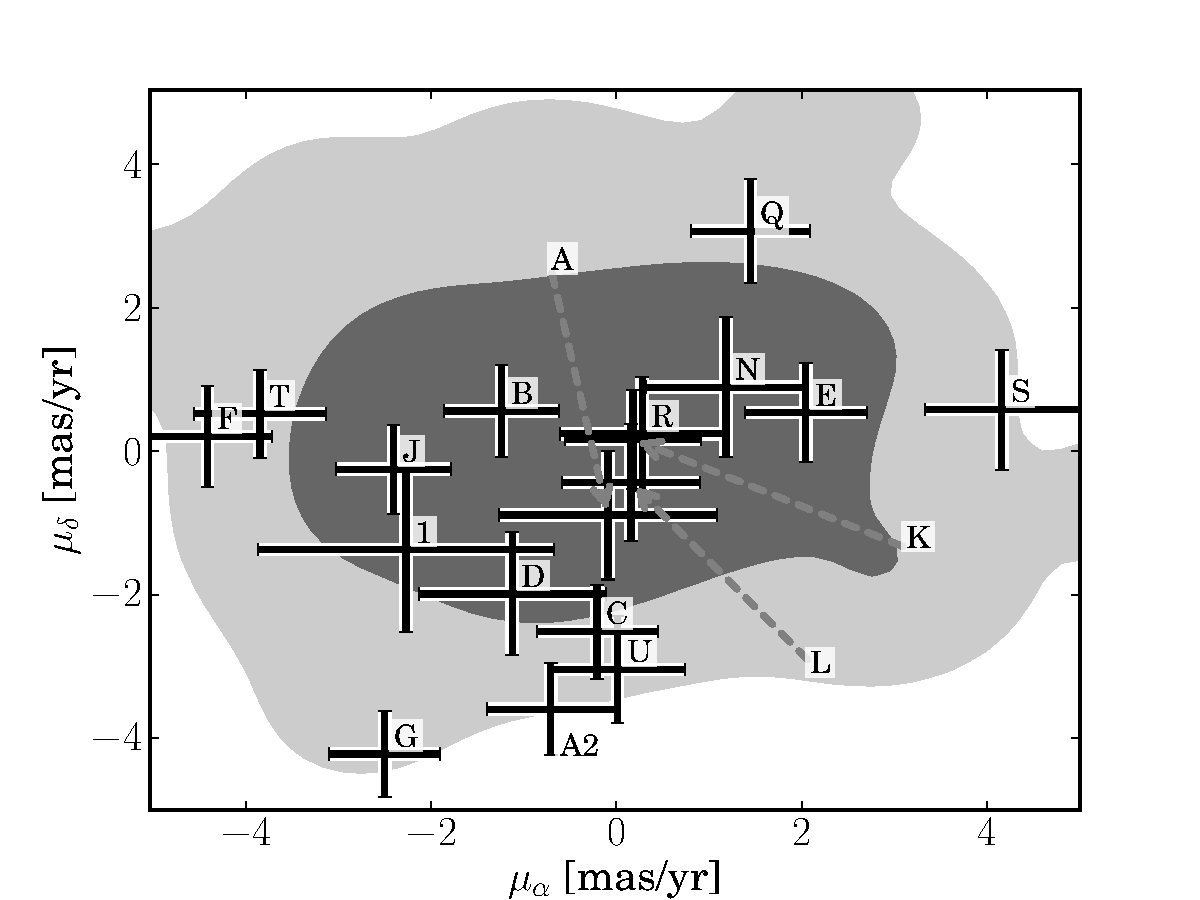
\includegraphics[width=0.5\textwidth]{chapter_sn1572_hires/plots/propmot_distr.pdf}
   \caption{The contours show the distribution of proper motion ($1-\sigma$ and $2-\sigma$) excluding the named stars.
    We show the location of the candidate stars and their errors on top of this distribution. Tycho-2 was not shown in this figure as it is an extreme outlier with $\mu_\alpha=75$\,\masyr\ and $\mu_\delta=-4.4$\,\masyr\ but also at a large distance to the center of the remnant's geometric center (46\arcsec).}
   \label{fig:propmot_sn1572_hires}
\end{figure}


\subsection{Radial Velocity}
\label{sec:radvel}

The radial velocity of each star was measured using the IRAF task \textit{fxcor} \citep{1979AJ.....84.1511T}. MAKEE was used to calculate an intrinsic velocity shift by comparing offsets of the nightsky-lines. The radial velocity standards were reduced in the same fashion. 
 
Each order of each star was then cross-correlated with at least two other radial velocity standards (HR6349, HR6970, HR1283) which had been observed on the same night.


The radial velocity for \starb\ was measured in the course of determining the stellar parameters for \starb\ with the stellar parameter fitting package \textit{sfit} \citesfit. The \textit{sfit} result consistently gives $v_{\textnormal{helio}} = -55$ \kms\ for different stellar parameters with an error of $\approx 2$\,\kms. 


In Table \ref{tab:radvel} we have listed all the radial velocities both in a heliocentric frame and a local-standard-of-rest (henceforth LSR) frame. We will be referring to the heliocentric measurements from here on. The listed error is the standard deviation of the radial velocity measurement of all orders added in quadrature to the error of the radial velocity standards.

In Figure \ref{fig:dist_vr} we have compared the radial velocity of our sample stars to radial velocities of stars in the direction of Tycho's SNR using the Besan\c{c}on Model \citep{2003A&A...409..523R}. The distance as well as the error in distance are taken from Section \ref{sec:distance}.  The candidates radial velocities are all typical for their distance. Finally, we note the measurement of \starg\ is consistent with \wek\ and \gh.

\ctable[
caption = {Radial velocities},
label = {tab:radvel},
]
{lccccc}{}{\FL
Name & Date & $v_{\rm helio}$ & $v_{\rm LSR}$ &$\Delta v$ \\
designation & (dd/mm/yy) & (\kms) & (\kms) & (\kms) \ML
%startdata
\stara & 09/09/06 & -36.79 & -28.5 & 0.23   \\
\starb & 09/09/06 & -55.0 & -57.0 & $\approx 2$ \\
\starc & 11/10/06 & -58.78 & -50.49 & 0.75   \\
\stard & 11/10/06 & -58.93 & -50.64 & 0.78   \\
\stare & 11/10/06 & -64.2 & -55.91 & 0.27   \\
\starg & 09/09/06 & -87.12 & -78.83 & 0.25 \\
\starg & 11/10/06 & -87.51 & -79.22 & 0.78 
\LL
}

\begin{figure}[htbp] %  figure placement: here, top, bottom, or page
   \centering
   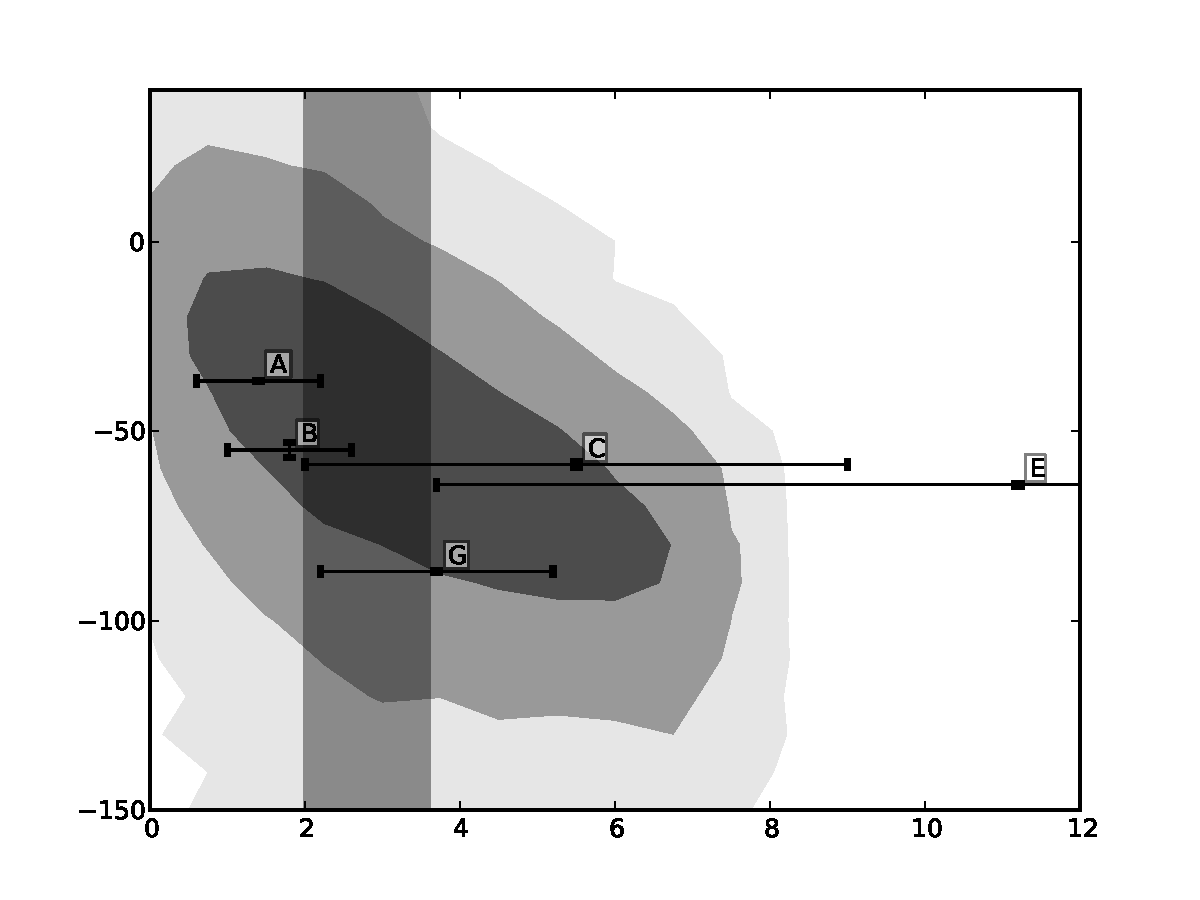
\includegraphics[width=0.5\textwidth]{chapter_sn1572_hires/plots/dist_vr.pdf} 
   \caption{The contours indicate 1, 2 and $3-\sigma$ levels of the distance and radial velocity using the Besan\c{c}on Model \citep{2003A&A...409..523R} with $\approx 60 000$ stars in the direction of SNR1572 (only including star with a V between 10 and 20 as well as stars with a metallicity of [Fe/H] $> -1$). We have overplotted our candidate stars with error bars. One should note that the errors in distance are only an indication of the error, the proper error surfaces can be seen in Figure \ref{fig:mc_isochrone}. The vertical gray shade shows the error range for the distance of SNR1572.}
   \label{fig:dist_vr}
\end{figure}



\subsection{Rotational Velocity}
\label{sec:rotation}
We have measured rotational velocities of all stars except \starb\ in the same fashion as described in \wek. We selected several unblended and strong (but not saturated) \ion{Fe}{1} lines in the stellar spectra .  We added these lines after shifting them to the same wavelength and scaling them to the same equivalent width. This was done to improve the signal to noise ratio for the faint stars as well as providing consistency throughout all stars. 

 As a reference we created three synthetic spectra for each star (one broadened only with the instrumental profile, the others with the instrumental profile and $v_{\rm{rot}}\sin{i}$\ of 10 and 13\,\kms\ respectively) with the 2010 version of MOOG \citemoog, using our derived temperature, gravity and metallicity.  As input data to MOOG we used the \citet{2004astro.ph..5087C} atmospheric models and a line list from \citet{1995KurCD..23.....K}. We then applied the same process of line selection and adding as for the lines in the observed spectra. 
 
Figure \ref{fig:rotvel} shows the comparison between the synthetic spectra of different rotational velocity and the observed spectra. This comparison indicates that the stellar broadening (rotational, macro turbulence, etc. ) is less than broadening due to the instrumental profile of 6\,\kms\ for each star. We adopt 6\,\kms\ as an upper limit to the rotation for all stars.



\begin{figure*}[h!]
\begin{tabular}{cc}
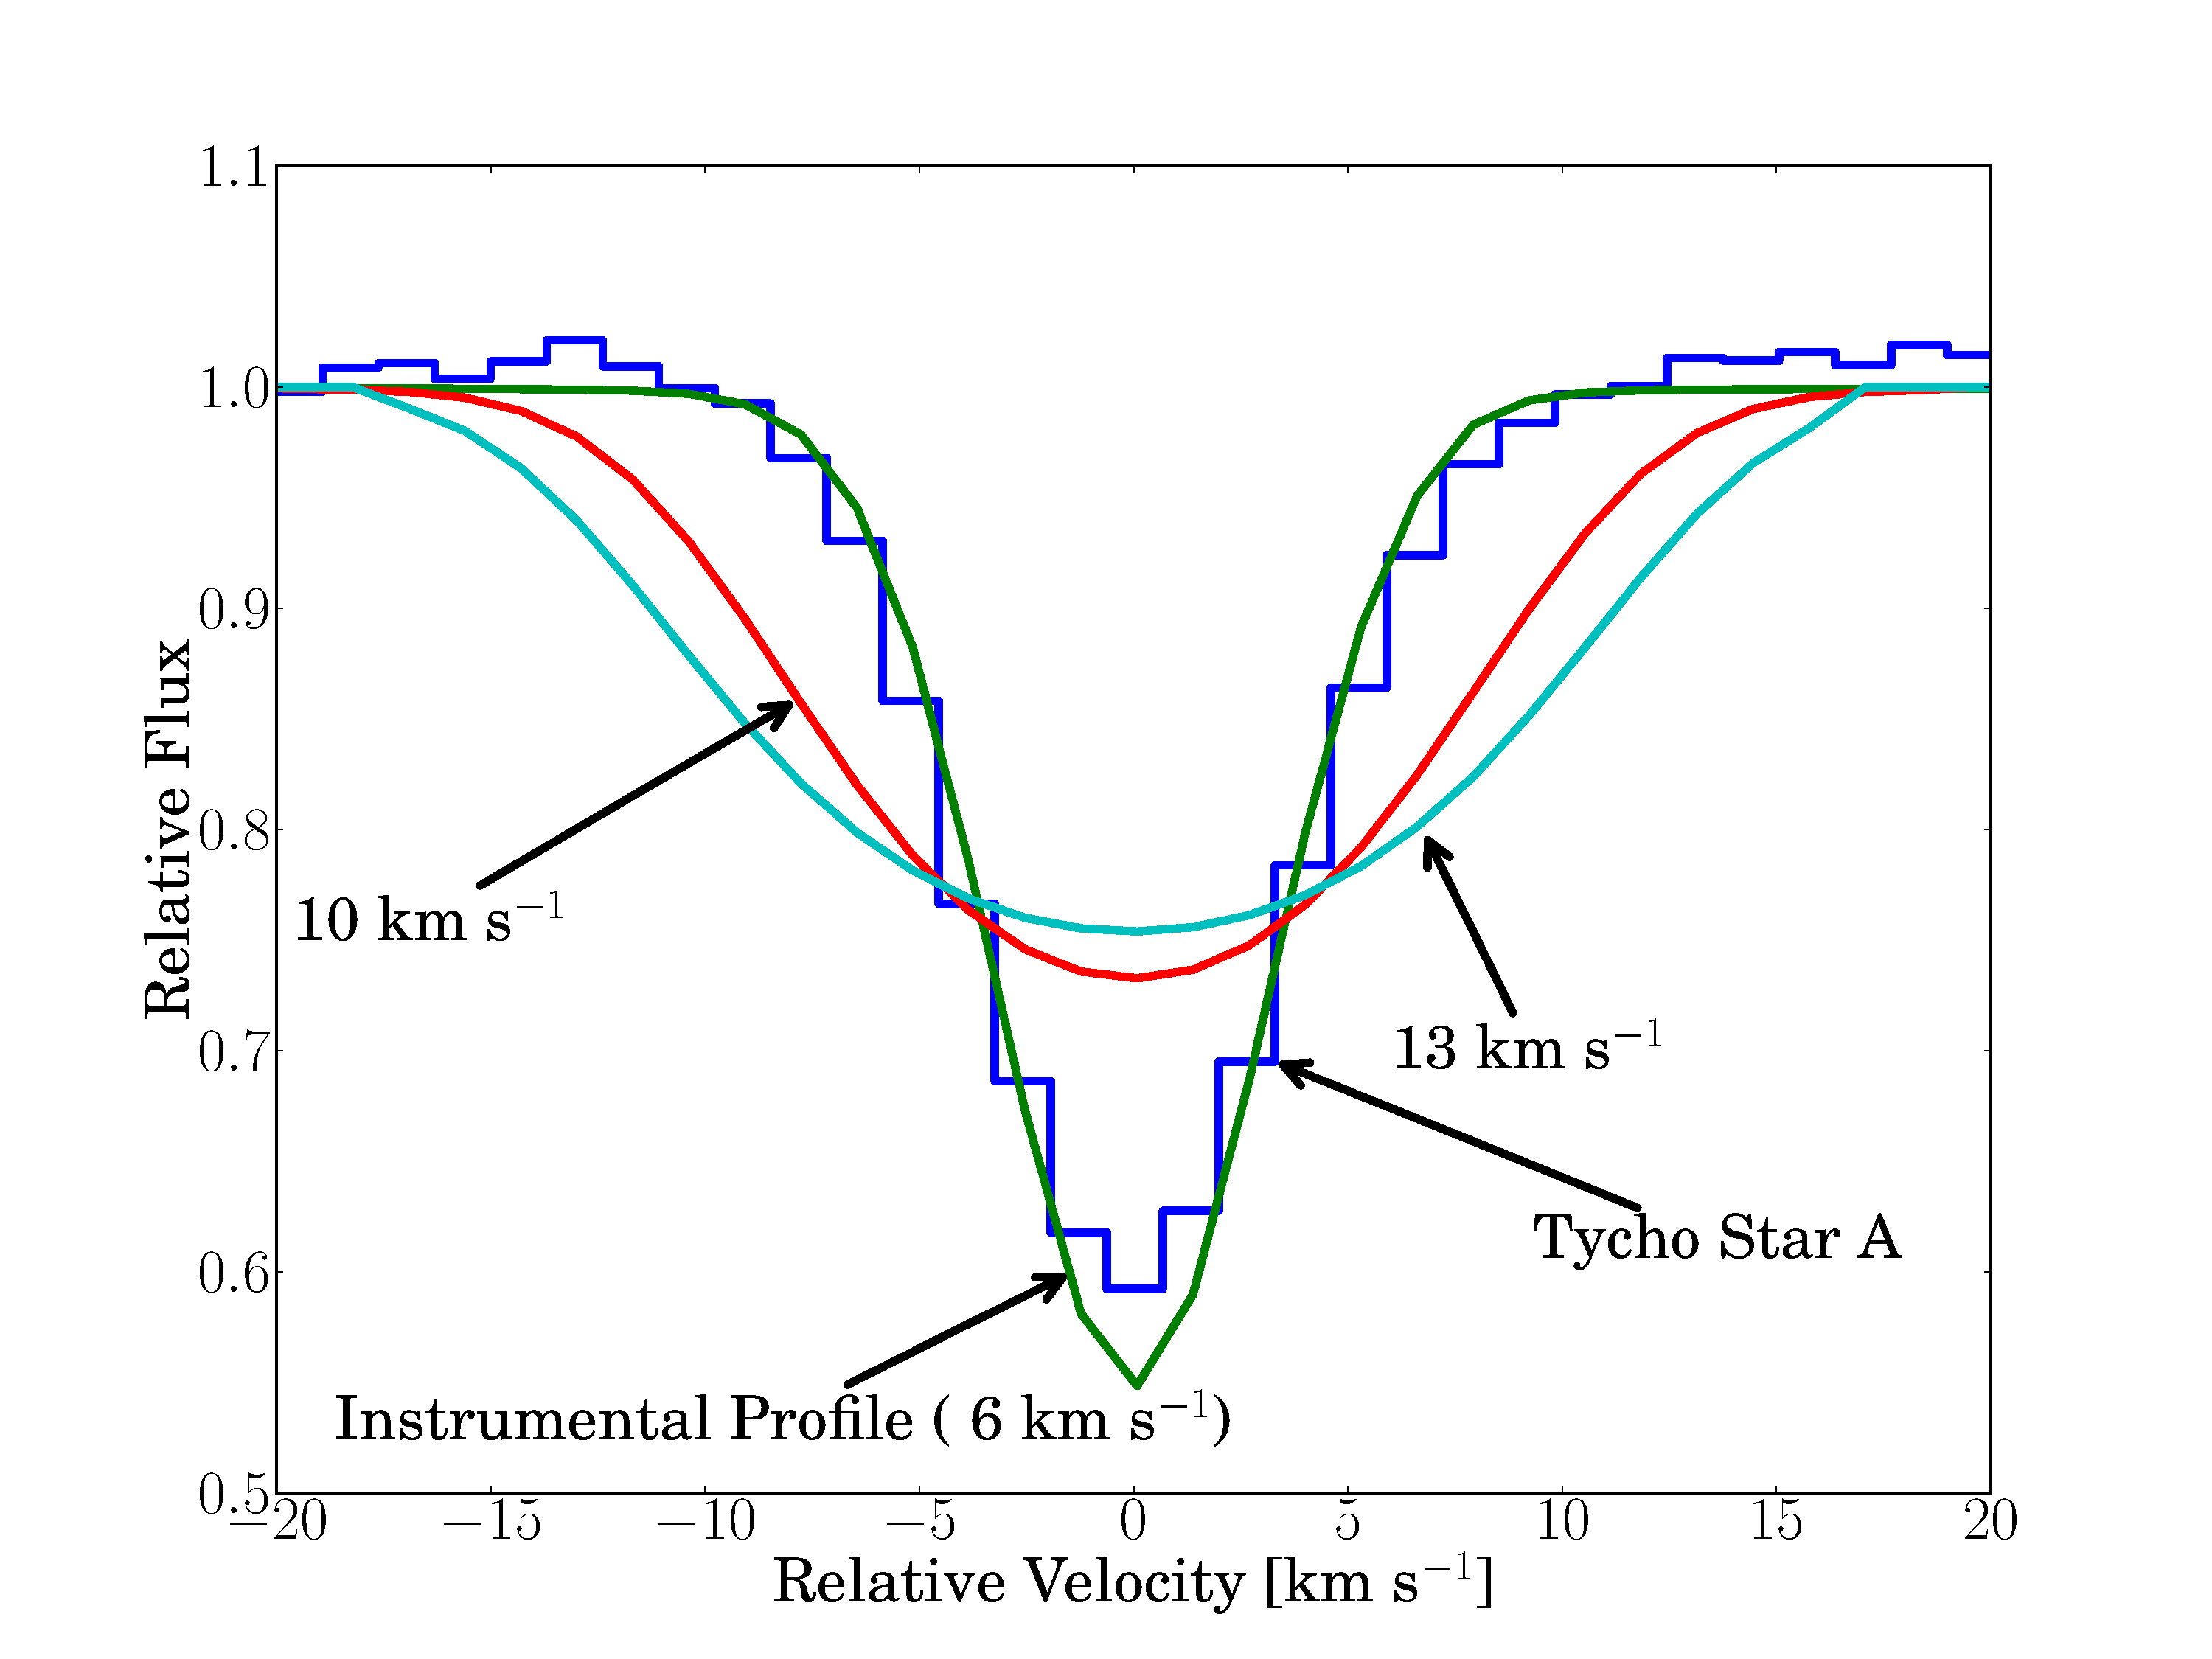
\includegraphics[width=0.45\textwidth, trim=130 30 60 0]{chapter_sn1572_hires/plots/stara_rotation.pdf} &
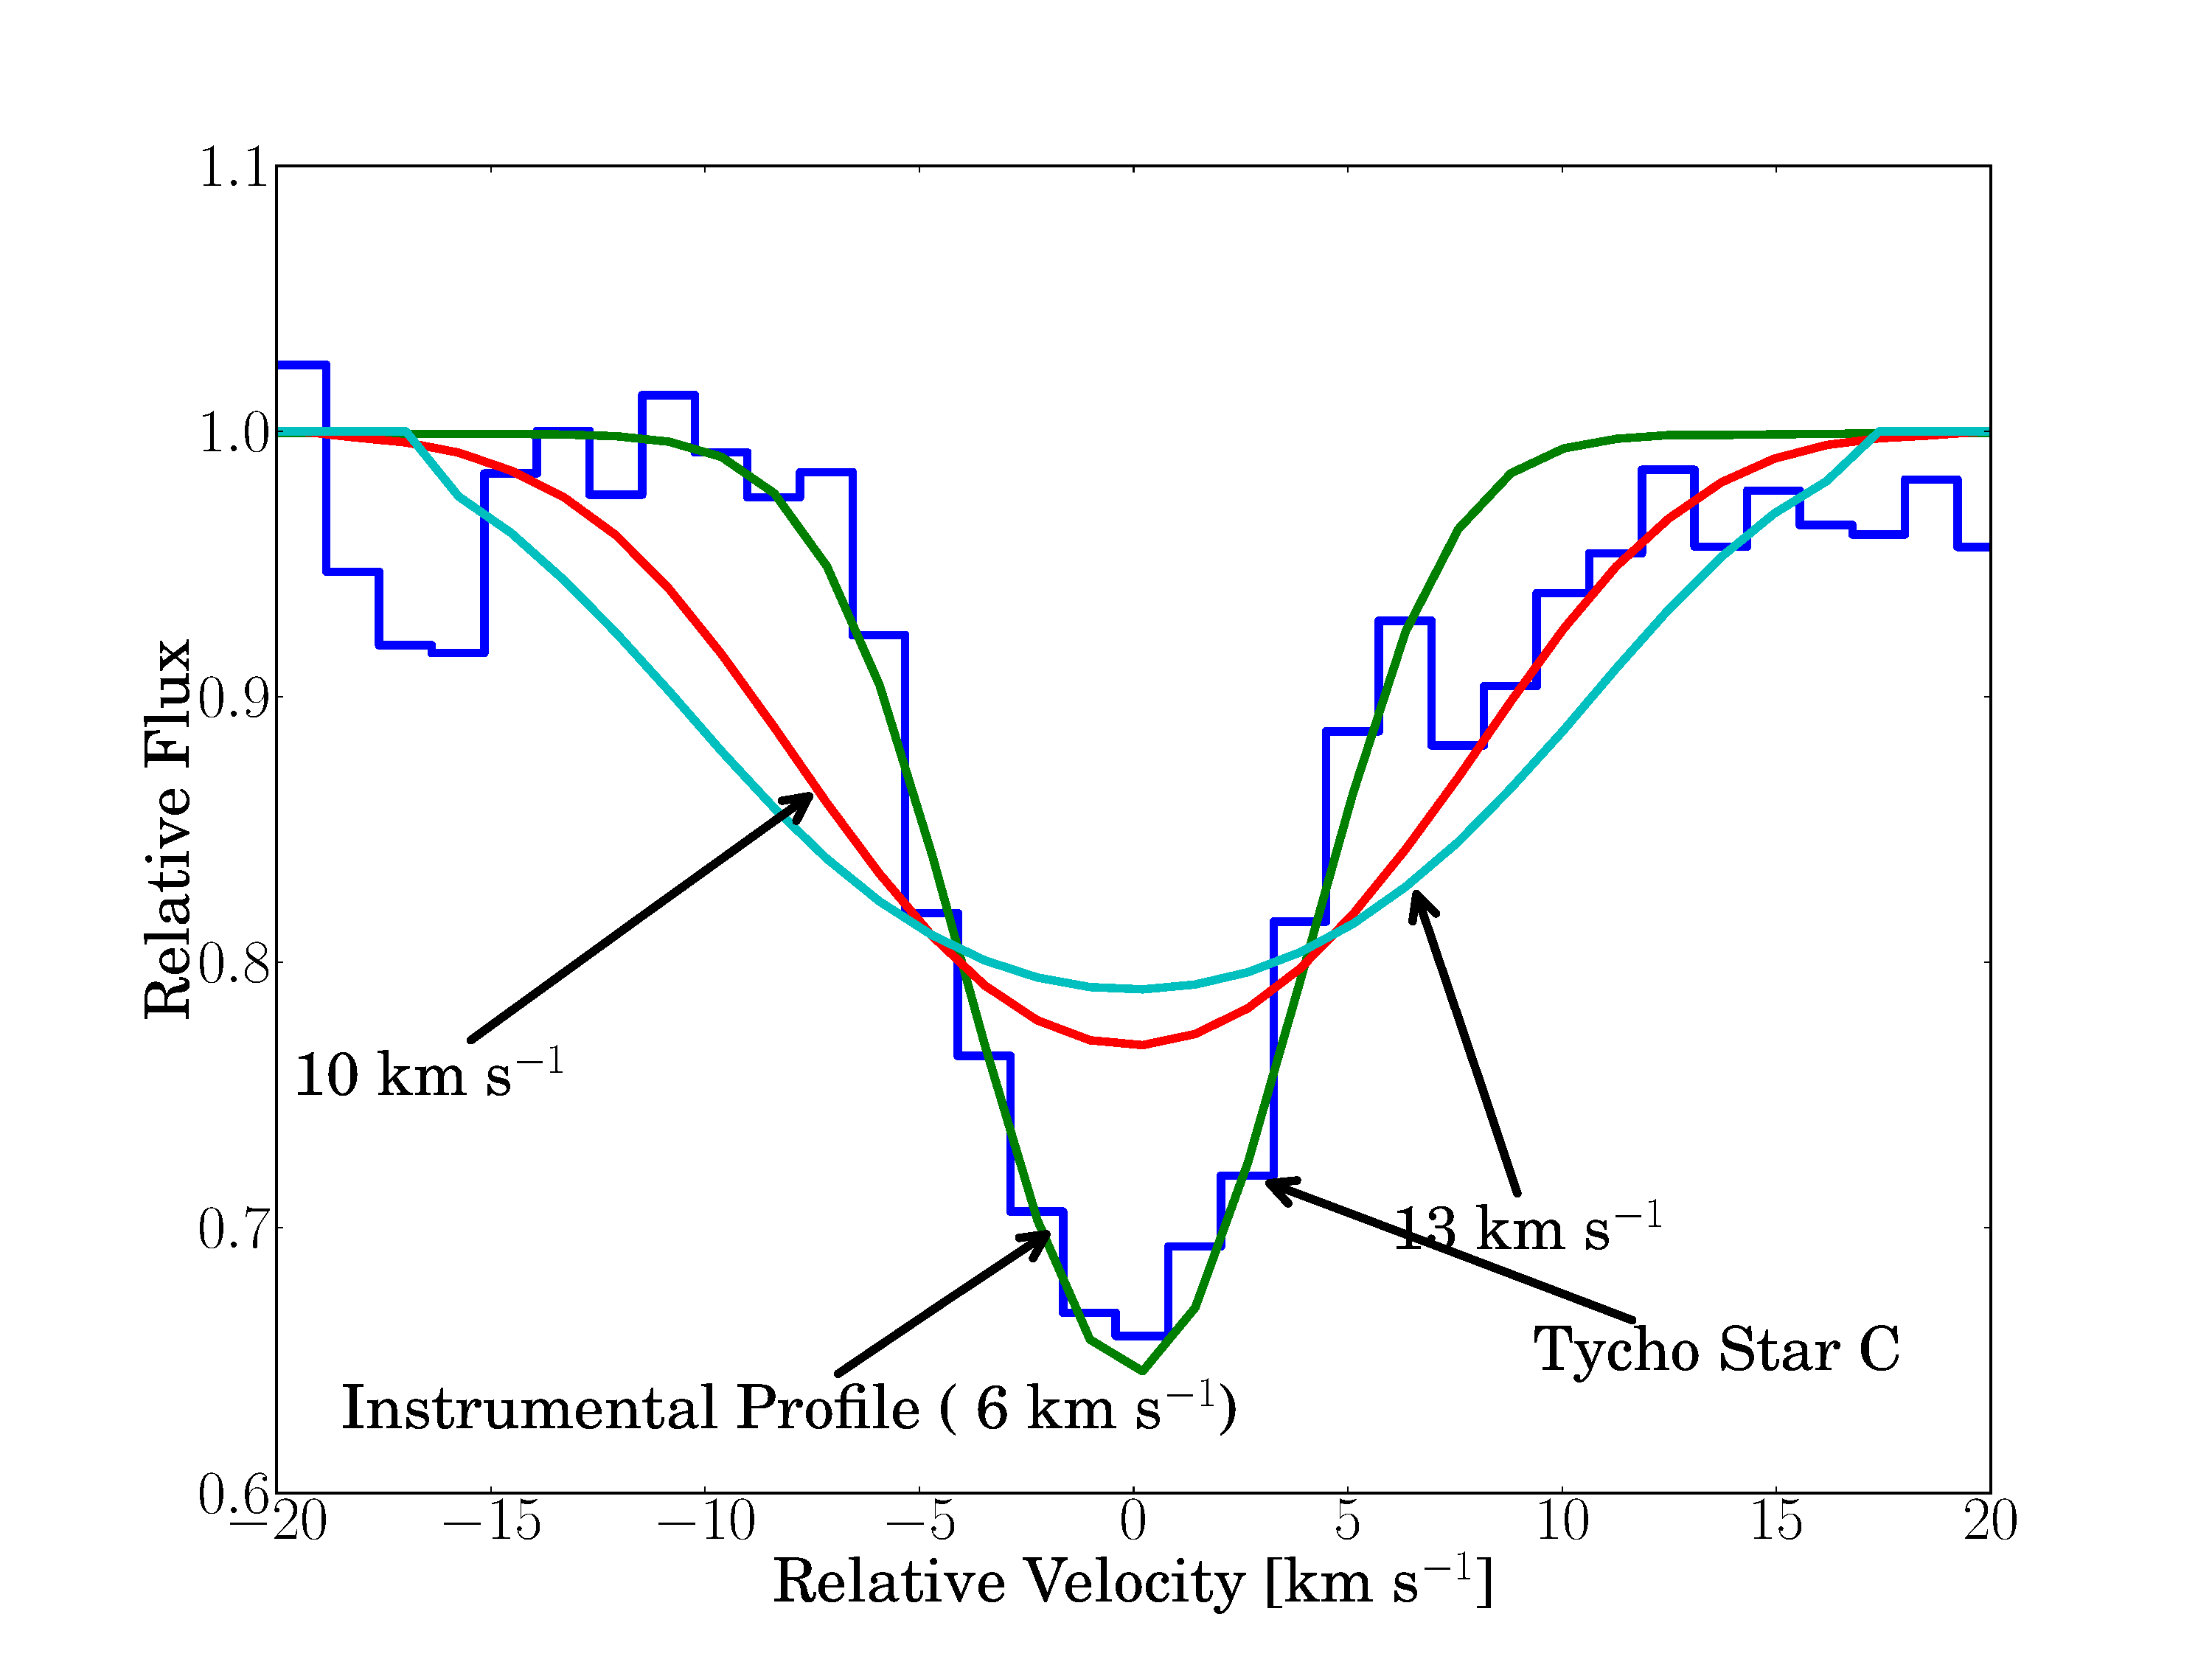
\includegraphics[width=0.45\textwidth, trim=130 30 60 0]{chapter_sn1572_hires/plots/starc_rotation.pdf} \\
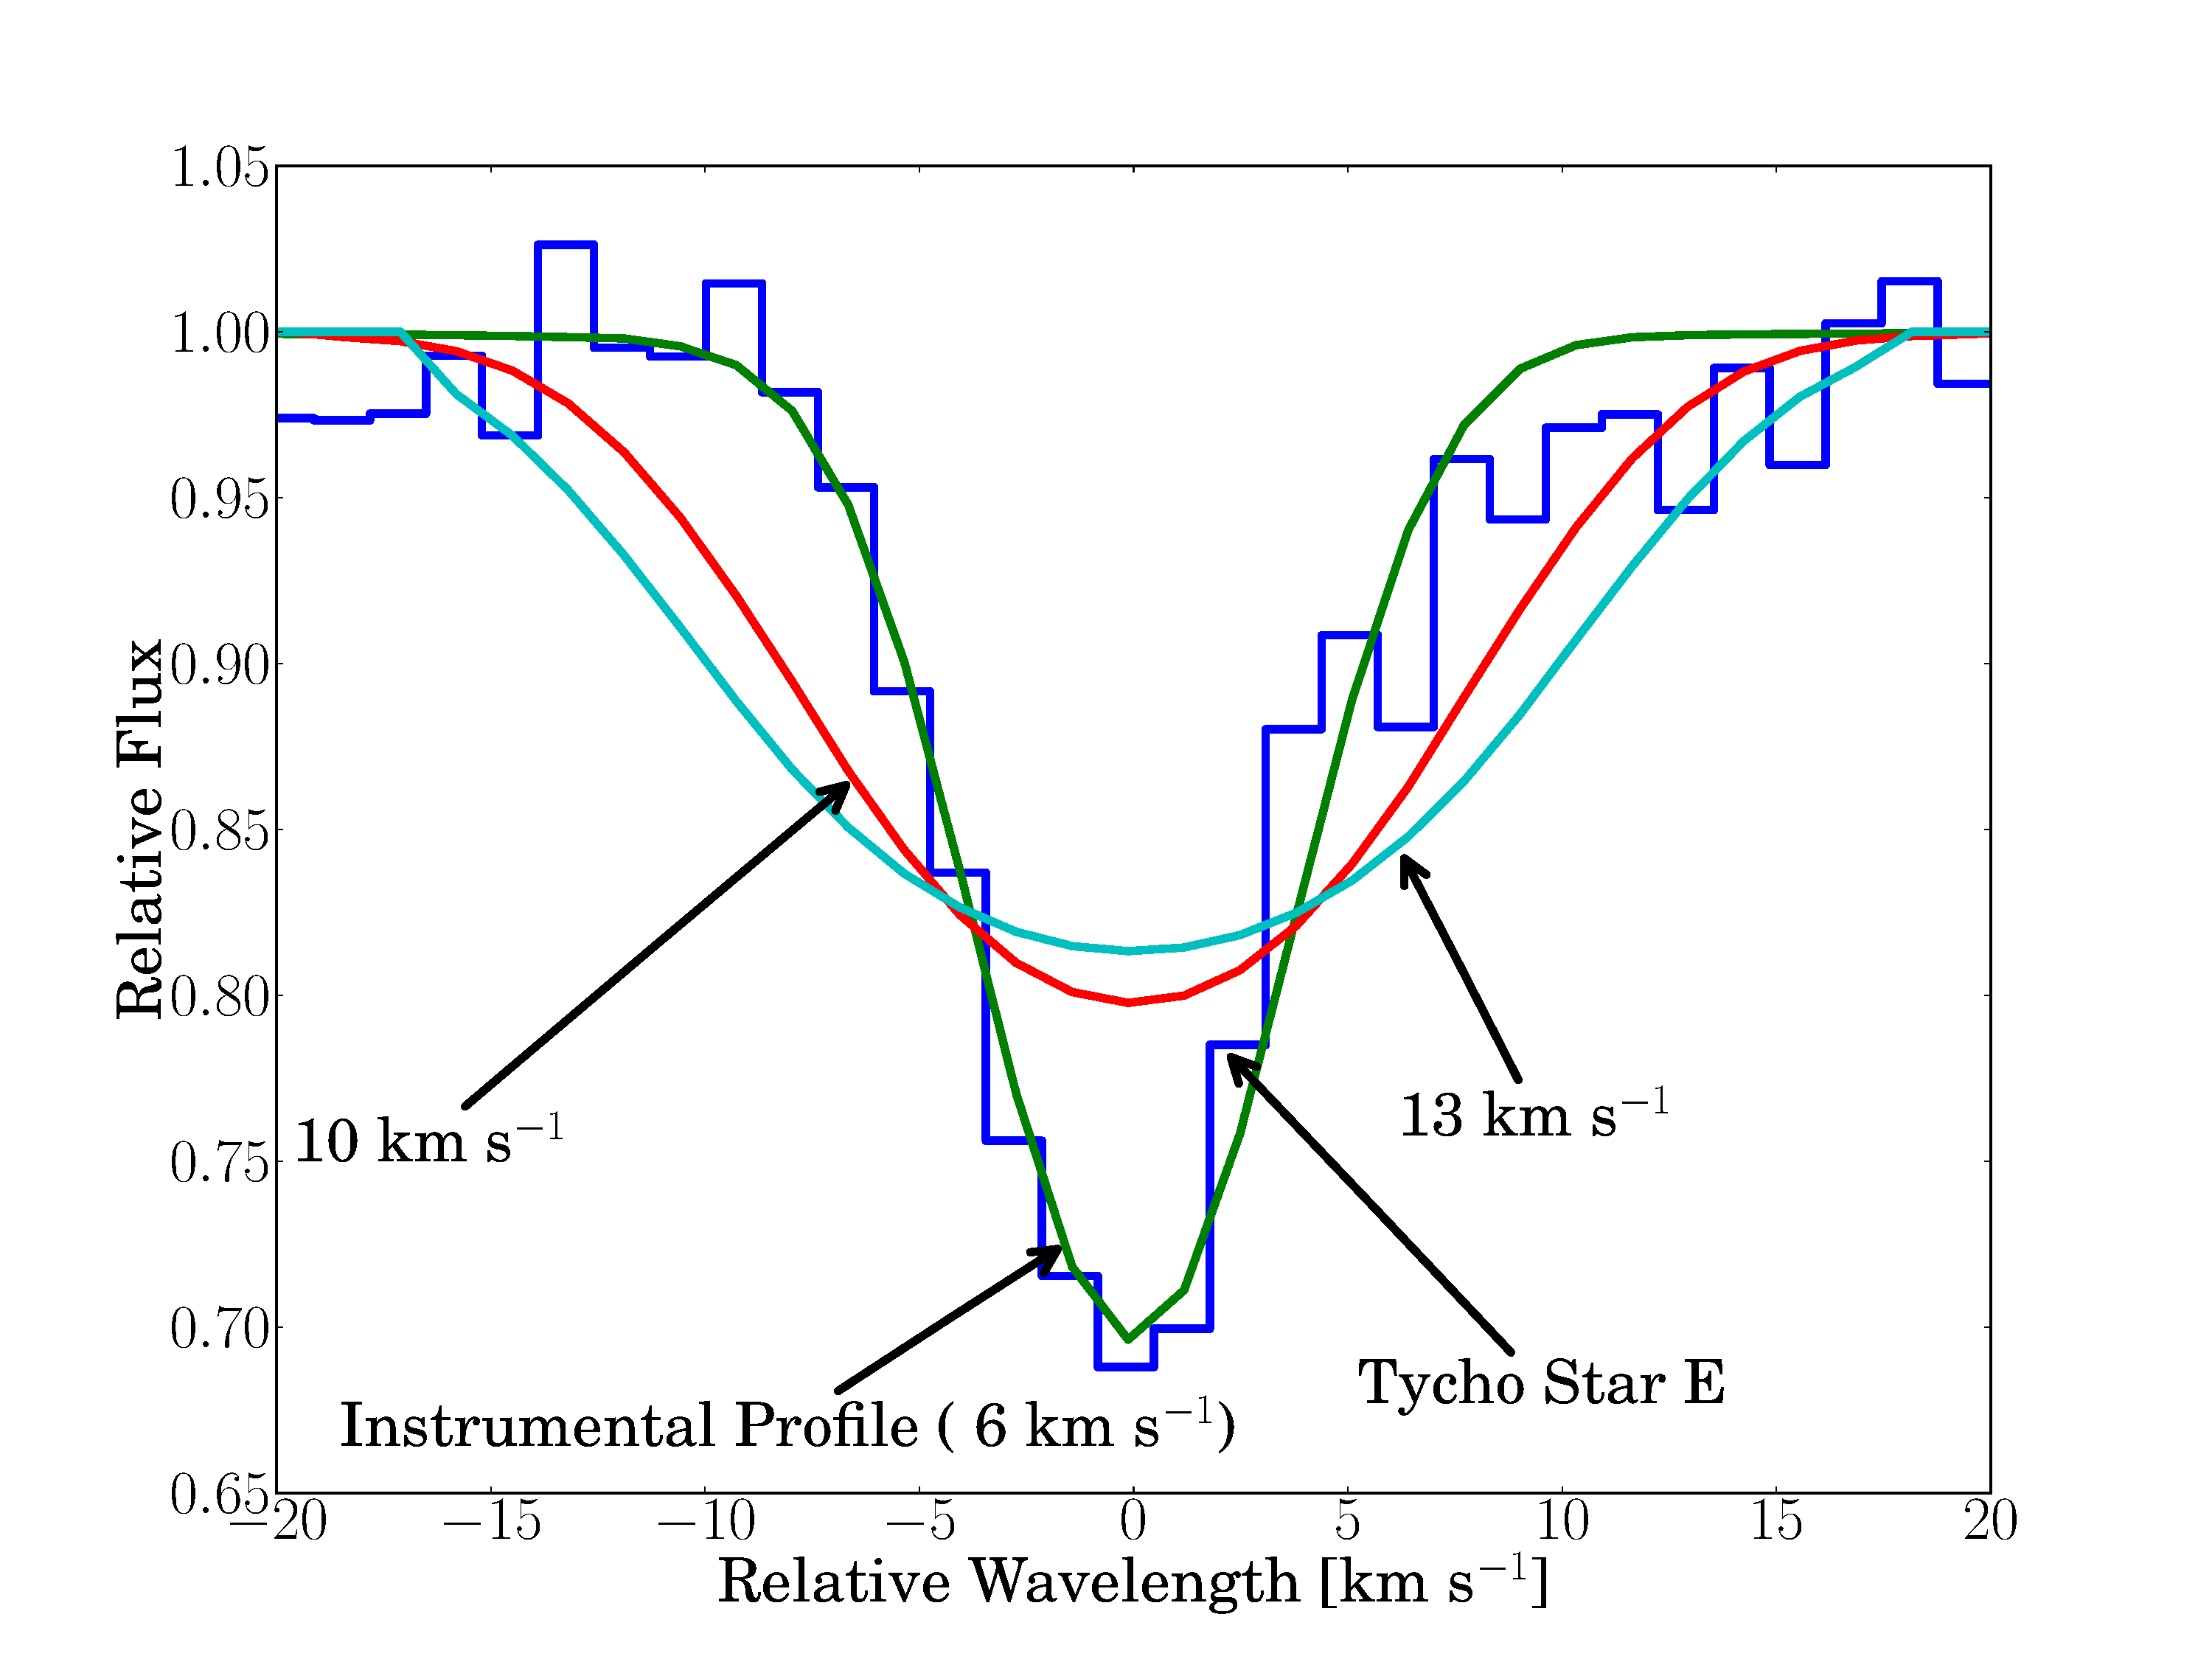
\includegraphics[width=0.45\textwidth, trim=130 30 60 0]{chapter_sn1572_hires/plots/stare_rotation.pdf} &
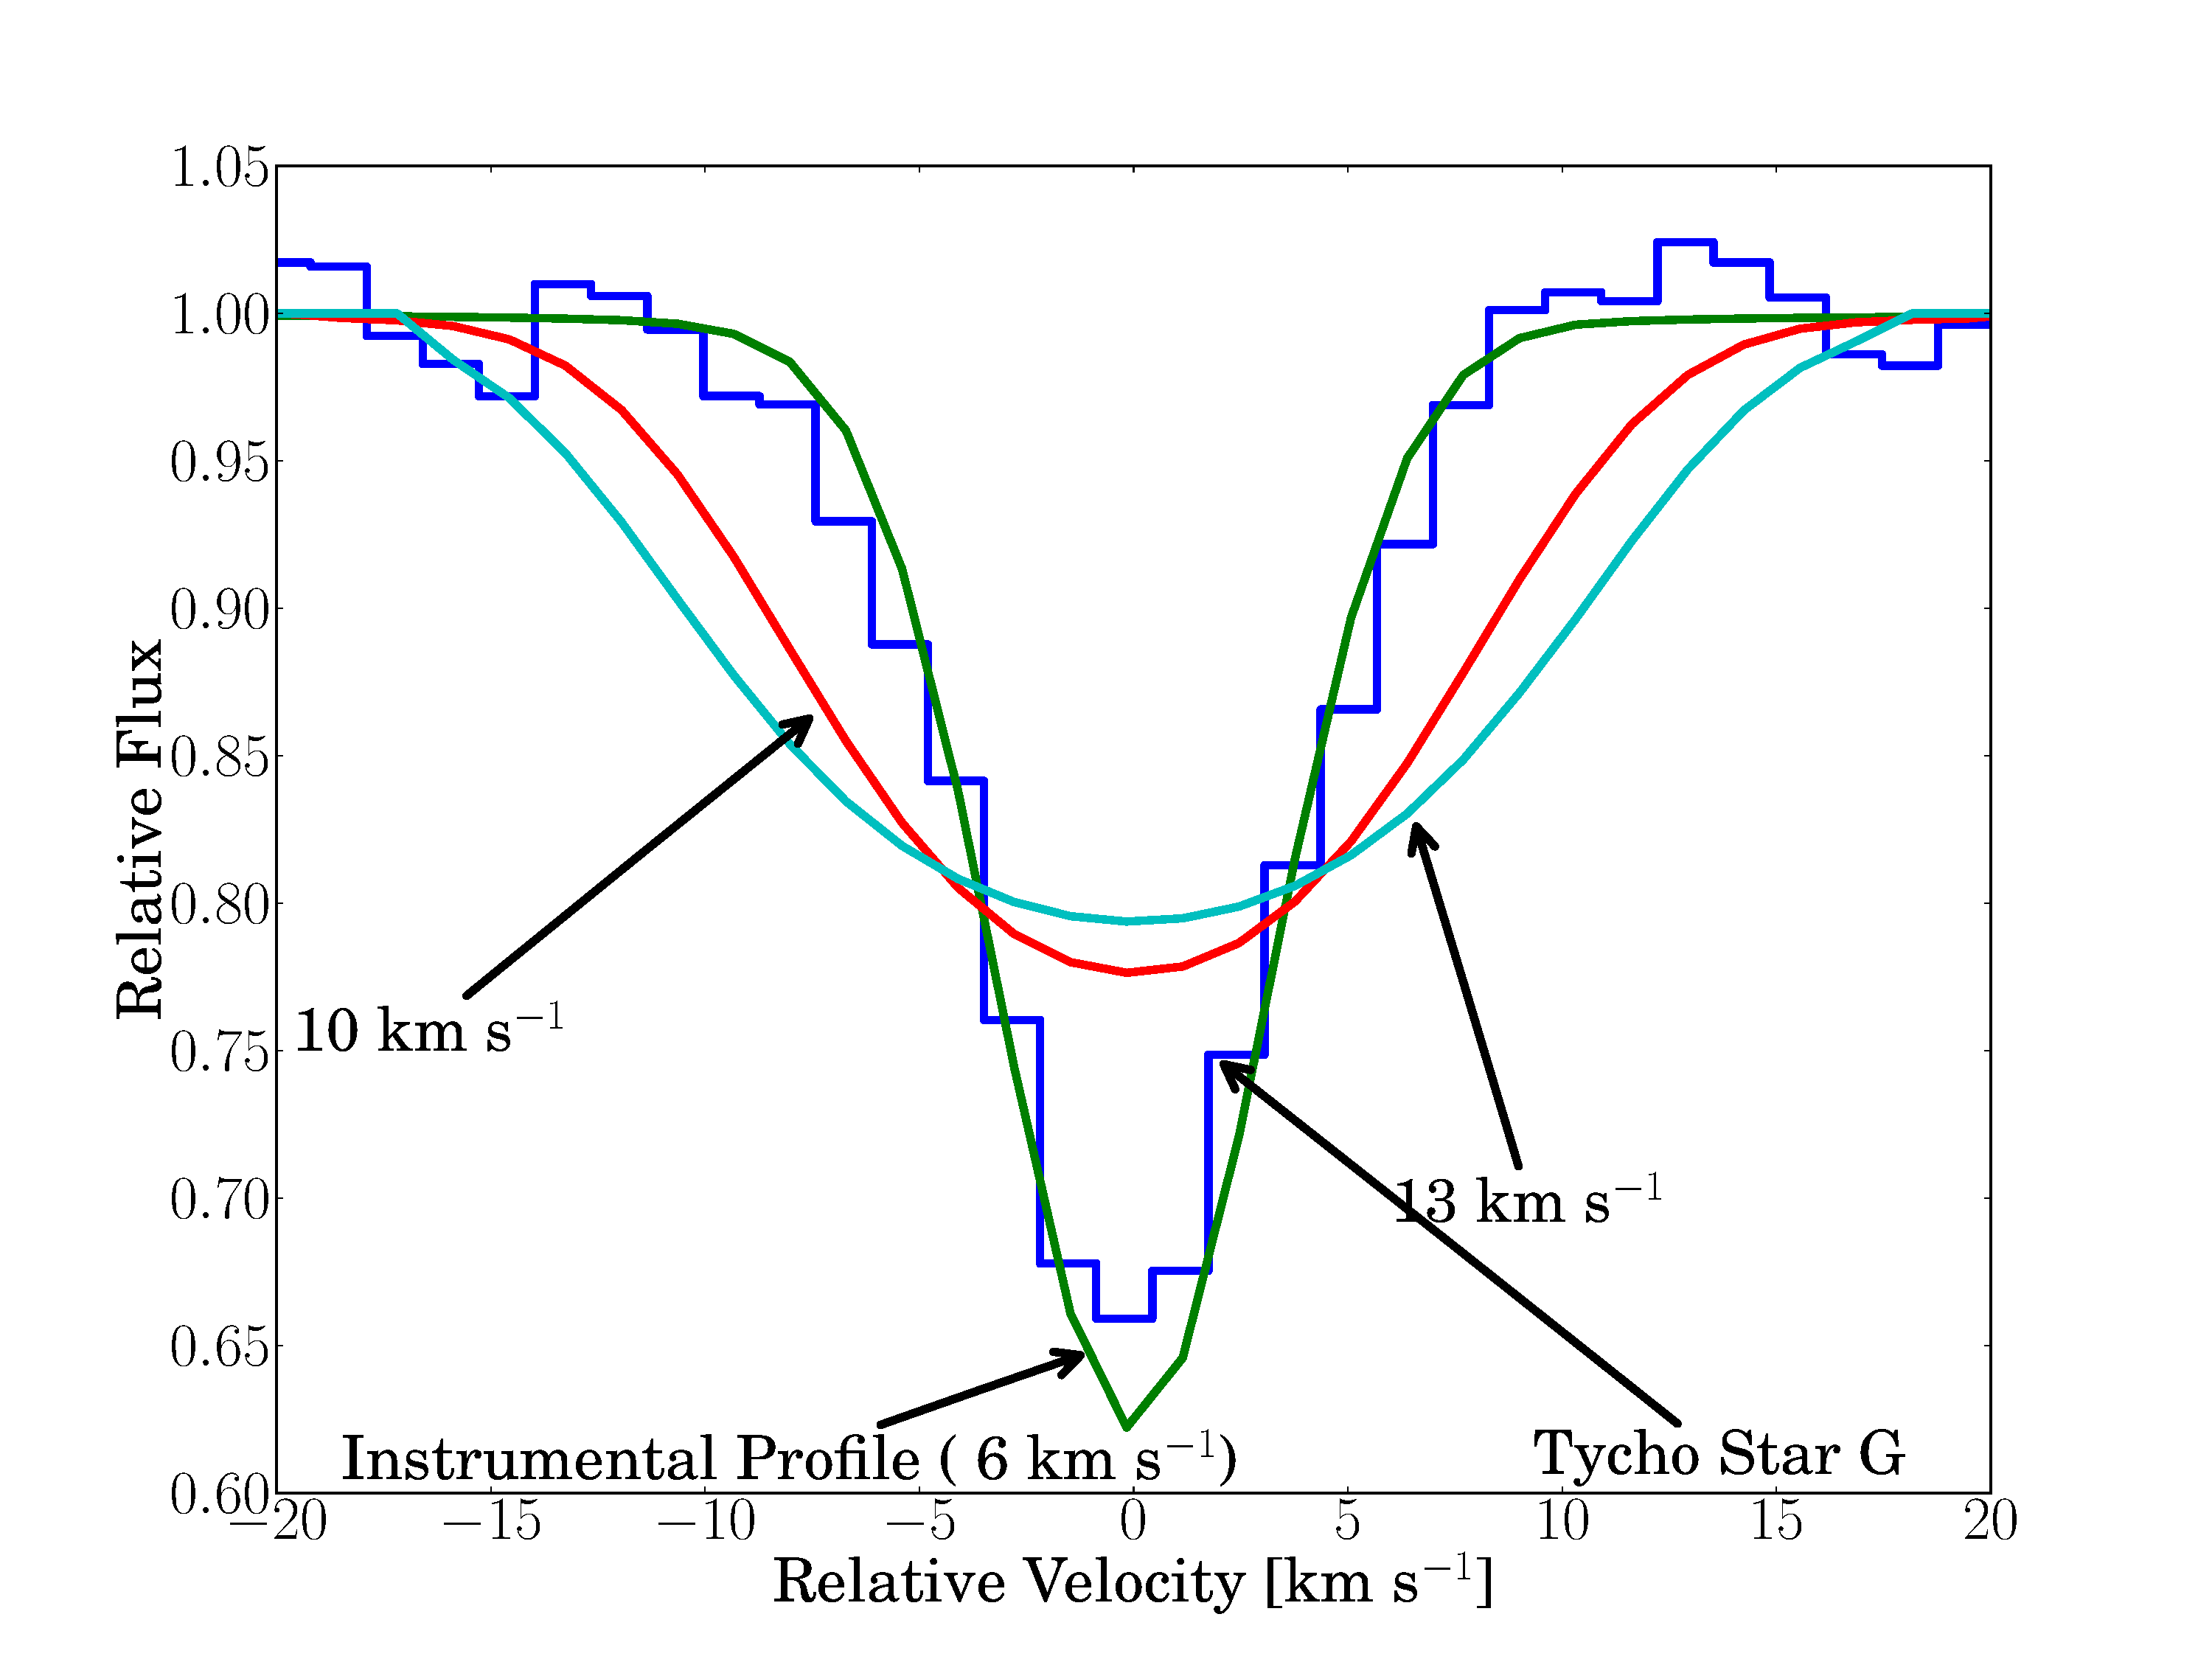
\includegraphics[width=0.45\textwidth, trim=130 30 60 0]{chapter_sn1572_hires/plots/starg_rotation.pdf} \\
\end{tabular}
\caption{The figures show the combination of Fe-line profiles after normalization to the same equivalent width and compare them to synthetic line profiles created by MOOG. We convolved the synthetic lines first with a rotational kernel with three different values for rotation and then with the instrumental profile. All stars show rotation less than 6 \kms\ which is equal to the instrumental profile at this resolution. }
\label{fig:rotvel}
\end{figure*}

Due to its high temperature and rotation, we fit the rotational velocity for \starb\ with the program \textit{sfit}\ \citep[][described in section \ref{sec:stellar-parameters}]{2001A&A...376..497J}  as part of the overall fit for this star's stellar parameters.  We find $v_{\rm rot}=171^{+16}_{-33}$\,\kms. While \starb's rotation is very high compared to the other candidate stars,  for stars of this temperature and gravity a high rotation is not unusual.


In summary, none of the stars show rotation which is measurable at this resolution.


\subsection{Stellar parameters}
\label{sec:stellar-parameters}
The stellar parameters are presented in Table \ref{table:stel_param} and were determined using a traditional spectroscopic approach based on the equivalent widths of lines of different excitation and ionization levels. . These measurements exclude \starb, due to its hot temperature, and we measure its stellar parameters by direct comparison to models, in a separate procedure.

Equivalent widths (EWs) for a set of Fe lines were measured using routines in IRAF (compiled from \citet[][henceforth Reddy03]{2003MNRAS.340..304R} and \citet[][henceforth RC02]{2002AJ....123.3277R} Table \ref{table:llist} shows the EWs measured for each of the stars. Missing values indicate that the line was not detected. 

We used the local thermodynamic equilibrium (LTE) stellar line analysis program MOOG \citemoog\ and LTE model atmospheres from the \citet{2003IAUS..210P.A20C} grid to derive an abundance for a given line. The effective temperature, \gls{teff}, was adjusted until the abundances from \ion{Fe}{1} lines displayed no trend as a function of excitation potential. The surface gravity, \gls{logg}, was adjusted until the abundances from \ion{Fe}{1} and \ion{Fe}{2} lines were in agreement. The microturbulent velocity, $\xi _{t}$ , was adjusted until there was no trend between the abundances from the \ion{Fe}{1} lines and EW. This process was iterated until self consistent stellar parameters were obtained  for each star. In our analysis, we explored stellar parameters at discrete values. For \gls{teff}, we considered values at every 25 K (e.g., 4000, 4025 K, etc.), for \gls{logg} , we considered values at every 0.05 dex (e.g., 1.00, 1.05 dex, etc.), and for $\xi _{t}$ , we considered values at every 0.05 \kms (e.g., 1.70, 1.75 \kms, etc.). We assumed that excitation equilibrium was satisfied when the slope between $\log{\epsilon}$(\ion{Fe}{1}) and lower excitation potential $(\chi)$ was $\leq0.004$. We assumed that ionization equilibrium was achieved when $\vert\log{\epsilon} ($\ion{Fe}{1}$) - \log{\epsilon} ($\ion{Fe}{2}$)\vert \leq 0.02$\,dex. The microturbulent velocity was set when the slope between $\log{\epsilon}$(\ion{Fe}{1}) and reduced equivalent width ($\log{\rm{W}}/\lambda$) was $\leq0.004$. In all cases we found appropriate solutions in which the trends between Fe I, Fe II, EW and excitation potentials were small. We estimate that the internal errors are typically $T_{\rm{eff}}\pm100$\,K, $\log{g}\pm0.3$\,dex, and $\xi _{t}\pm0.3$\,\kms. 
For further details regarding the derivation of stellar parameters, see \citet{2008ApJ...673..854Y}.

The final iron measurements are the average of \ion{Fe}{1} and \ion{Fe}{2} assuming the solar abundances of \citet{2009ARA&A..47..481A} 
In addition, we measured abundance for the Elements Ni and Li via EW analysis. We could not see any unusual abundance pattern for any of the sample stars (see Figure \ref{fig:kobayashi06}; \starb's abundances are not presented on the plot as they were measured in a different fashion).  


\ctable[
caption = {Stellar Parameters},
label = {tab:stel_param}
]
{lccccccc}{}{\FL
Name & \gls{teff} & \gls{logg} & \gls{feh} & $\Delta$\gls{feh}& [Ni/H] & $\Delta$[Ni/H] & [Li/H] \\ 
designation & (K) & (dex) & (dex) & (dex) & (dex) & (dex) & (dex) \ML 
%\startdata
\stara & 4975 & 2.9 & 0.02 & 0.16 & 0.05 & 0.025 & 0.09 \\
\starc & 4950 & 2.9 & -0.57 & 0.23 & -0.14 & -0.17 & 0.11 \\
\stare & 5825 & 3.4 & -0.16 & 0.21 & 0.2 & 0.0 & 0.131\\
\starg & 6025 & 4 & -0.15 & 0.18 & 0.14 & 0.08 & 0.11 \LL
}

\begin{figure}[h] %  figure placement: here, top, bottom, or page
   \centering
   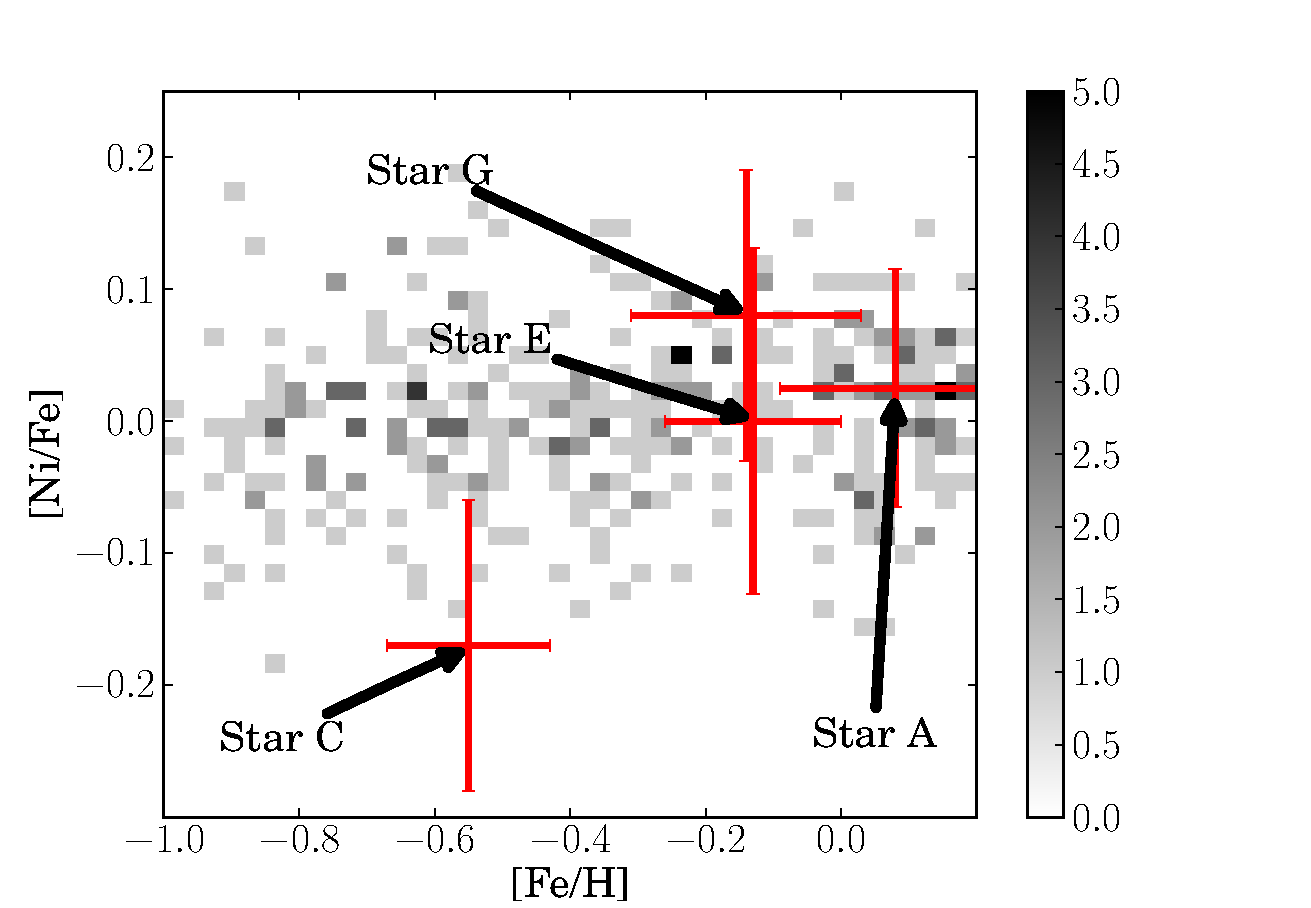
\includegraphics[width=1\textwidth]{chapter_sn1572_hires/plots/abund_chiaki.pdf} 
   \caption{The background colour indicates the distribution is taken from \citet{2006ApJ...653.1145K}. All of the measured candidates are consistent within the errors with stars of the same metallicity.}
   \label{fig:kobayashi06}
\end{figure}

In summary, the inferred metallicities for all candidates show that the candidates are of roughly solar metallicities with the exception of the metal-poor \starc. The range of metallicities spanned by the program stars is compatible with membership of the thin disk (REFERENCE). Based on metallicity alone, we do not regard any of the program stars to be unusually metal-poor or metal-rich.  Additionally, we find the [Ni/Fe] abundance to be consistent with stars of similar metallicity (see Figure \ref{fig:kobayashi06}). The stellar paramaters and elemental abundances are listed in Table \ref{tab:stel_param}.

Because Tycho B has a temperature  greater than 9000 K and is quickly rotating, the process described above cannot be used to measure stellar parameters. Instead we used the program \textit{sfit}\ \citesfit\ to match the HIRES-spectrum to a grid of model spectra. To determine the stellar parameters for \starb\ we have used a model grid with $\textnormal{[Fe/H]} = -1.0$, $8000 < T_{\textnormal{eff}} < 16000$, $7 < \log{g} < 2$. This low metallicity is suggested by a very weak Calcium K line and Mg II lines, but is hard to measure. We can not measure Helium directly in this spectrum and thus adopt N(He) = 0.1 as this is empirically a very common Helium abundance in stars.

This analysis resulted in $T_{\rm eff} = 10000^{+ 400}_{-200}\,\rm{K}$, $\log{g} = 3.67$ with slope  $\partial \log{g}/\partial T_{\rm eff} = 0.27/500 \,\rm{K}^{-1}$, rotational velocity $v\sin{i} = 171$\,\kms\ with slope $\partial v\sin{i}/\partial T_{\rm eff} = -41/500\,\rm{km\,s^{-1}\,K^{-1}}$. From qualitative analysis this object seems metal poor (e.g. in comparison to stars of similar stellar parameters but solar metallicity), but its high rotation and temperature make it hard to determine this parameter precisely. For the present, we assume [Fe/H] = -1.0 unless otherwise noted.

In addition, using the high-resolution spectrum, we measured the equivalent widths of several lines predicted to be strong in the VALD database \citep{2000BaltA...9..590K}. The abundances were deduced from the equivalent widths using a model atmosphere having $T_{\rm eff} = 10000$\,K, $\log{g}=3.67$ and [Fe/H] = -1.0 (see Table \ref{tab:starb-abund}).

One caveat regarding these abundances is the use of equivalent widths from 
single lines with large rotational broadening, since the effect of blending 
with nearby weak lines cannot be taken into account. A second is that these 
abundances invariably rely on the strongest lines, which are precisely those 
most susceptible to departures from local thermodynamic equilibrium. 
Nevertheless, they do confirm the earlier impression that the star is 
metal-poor, and justify the adoption of [Fe/H]=$-1.0 \pm 0.4$.

%ctable goes here
\ctable[
caption={\starb\ abundances},
label={tab:starb-abund},
]
{lcccccc}{}{\FL
Ion&$\lambda$& $W_{\lambda}$& $\epsilon$& $[X/H]$ & $\frac{\partial \epsilon}{\partial \log{g}}$  &$\frac{\partial \epsilon}{\partial T_{\rm eff}}$\\
designation & \AA & \AA & dex & dex& &K$^-1$ \ML
%\startdata
\ion{Mg}{2} & 4481.13+4481.33 & $220\pm15$ & $6.18\pm.08$ & -1.40&0.08&$8\times10^{-5}$ \\ 
\ion{Si}{2} & 6347.1 & $140\pm5$ & $6.96\pm.18$ & -0.59&-0.02&$1\times10^{-4}$\\
\ion{O}{1} & 7771.9+7774.2+7775.4 & $460\pm30$ & $8.43\pm.10$ & -0.58 &0.24&$-4\times10^{-5}$ \LL
}


As a second approach to determine the stellar parameters of \starb\ we used the low resolution spectra observed with LRIS.  The observation range of LRIS was chosen to be centered around the Balmer jump as this feature is sensitive to the surface gravity \citep{2007PASP..119..605B}. We fitted the spectra to a grid of model spectra \citep[]{2005A&A...442.1127M} using a spectrum fitting tool  described below. The final grid we used covered $\log{g}$ from 3.5 to 4.5 in steps of 0.5 and \gls{teff} from 9000 to 12000\,K in steps of 500\,K. In addition we expanded the grid by reddening the spectra with the \textit{pysynphot}-package\footnote{pysynphot is a product of the Space Telescope Science Institute, which is operated by AURA for NASA.}. We also added diffuse interstellar bands  \citep{1937PASP...49..224B, 1966ZA.....64..512H, 1967IAUS...31...85H, 1975ApJ...196..129H, 1995ARA&A..33...19H, 1994dib..nasa...31H, 1994A&AS..106...39J, 1958ApJ...128...57W} to the synthetic spectra , which were scaled with reddening . The included E(B-V) ranged from 0.5 to 1.3 in steps of 0.2. We assumed a rotation of 171\,\kms\ in the grid  (see section \ref{sec:rotation}).

We used $\chi^2$ as a figure of merit in our fitting procedure. To find the best fit for \starb\ we used the MIGRAD algorithm provided by \textit{MINUIT} \citep{James:1975dr} and linearly interpolated between the grid points using \textit{LinearNDInterpolator} provided by the \textit{scipy}-package  \cite{Jones:2001fk}. The fit of \starb\ results in \gls{teff}=10570\,\textrm{K}, \gls{logg}=4.05, \gls{feh}=-1.1 and E(B-V)=0.85. The model fits the synthetic spectrum poorly  in the wavelength region between 3800 -- 4280 \AA\ in (see Figure \ref{fig:starb_spec_comp}). The adopted mixing length parameter used in 1D model atmospheres used to construct the spectralgrid influences the fluxes in that region as well as affecting the hydrogen line profiles. \citet{2002A&A...392..619H} and others show that a mixing length of 0.5, rather than 1.25 as used in the Kurucz/Munari grid, better fits the violet fluxes and the hydrogen line profiles. Spectra using a mixing length parameter of 0.5 are brighter in the violet and the $\textrm{H}_\gamma$, $\textrm{H}_\delta$ and $\textrm{H}_\beta$ profiles give the same \gls{teff} as the $\textrm{H}_\alpha$ profiles. We have chosen, however, to fit the spectrum and ignore the problematic spectral region (3800 -- 4280 \AA) to avoid a systematic error. This yields \gls{teff}=10722\,K, \gls{logg}=4.13, \gls{feh}=-1.1 and E(B-V)=0.86. The differences are indicative of a systematic error in the model. We adopt the fit excluding the problematic wavelength region in the further analysis. Exploring the complex search space we estimate the error to be $\Delta\gls{teff}$=200\,K, $\Delta\gls{logg}$=0.3 and $\Delta\gls{feh}$=0.5, but acknowledge that the parameters are correlated.  



\begin{figure*}[h!]

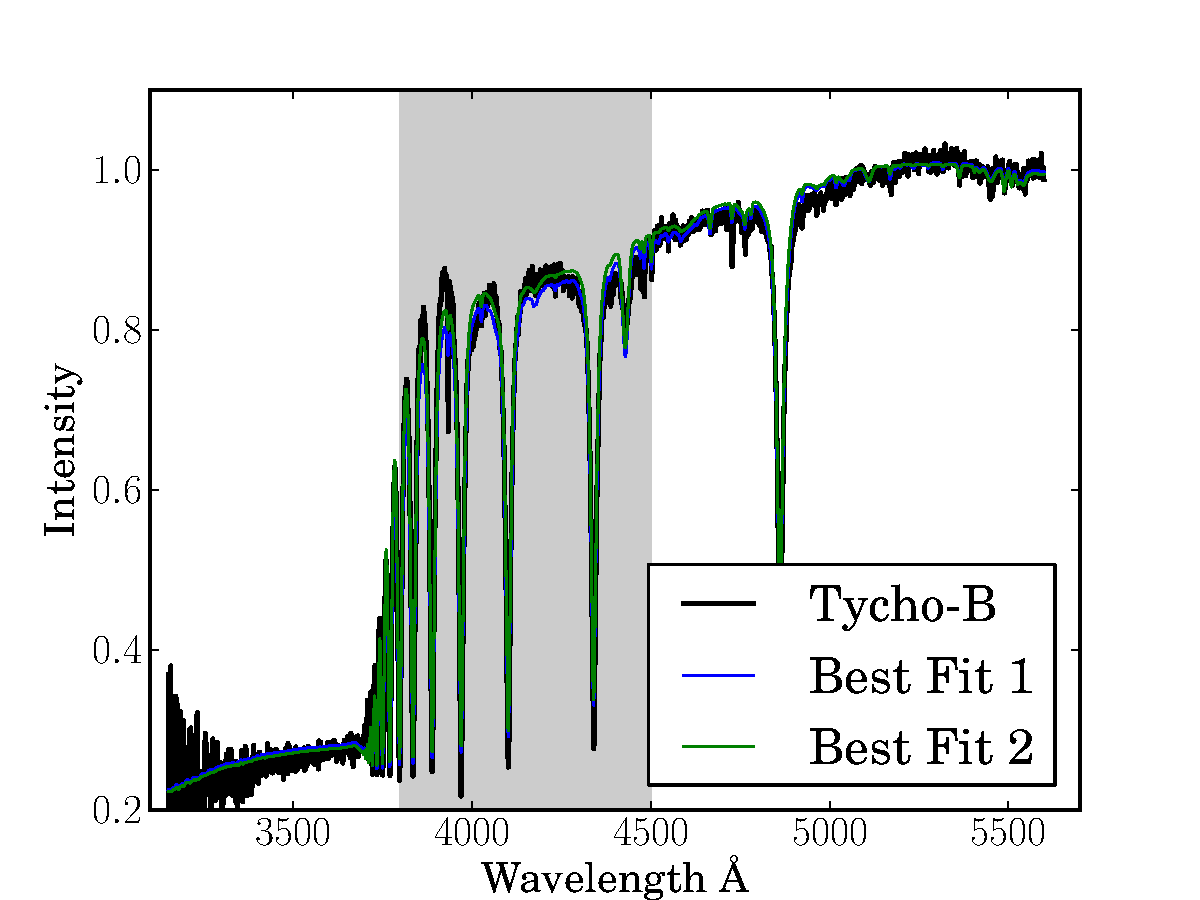
\includegraphics[width=1.\textwidth]{chapter_sn1572_hires/plots/starb_spec_comp.pdf} 

\caption{The plot shows the normalized spectrum of \starb\ with the fit which excluded the spectral region between 3800 -- 4500 \AA (Best Fit 1) and the fit with the problematic region (Best Fit 2). The region is marked with a gray shade.  }
\label{fig:starb_spec_comp}
\end{figure*}

\subsection{Distance}
\label{sec:distance}
To measure the distance to the candidate stars we used colours and absolute magnitude from isochrones by  \citet{2004ApJ...612..168P}. We used the MIGRAD algorithm  \citep{James:1975dr} to find close matches of the measured values to \gls{teff}-\gls{logg} isochrones by varying the age of the isochrone.  Subsequently we calculate E(B-V) using the isochrone's colour and we extract a mass from the isochrone. The results can be seen in Table \ref{table:iso_dist}. To estimate the errors in all distance, reddening and mass we employed the Monte-Carlo
method with 10,000 samples of \gls{teff} , \gls{logg}, \gls{feh}, B- and V-magnitude (see Figure  \ref{fig:mc_isochrone}).  Errors included in Table \ref{table:iso_dist} are the standard deviations of the Monte-Carlo sample. 
The data shows that all stars are compatible with the distance of the remnant. This is not unexpected as the uncertainties of the measurements in stellar parameters are relatively large.




\begin{figure}[htbp] %  figure placement: here, top, bottom, or page
   \includegraphics[width=0.5\textwidth]{chapter_sn1572_hires/plots/tycho-a-panel.pdf} 
   \includegraphics[width=0.5\textwidth]{chapter_sn1572_hires/plots/tycho-b-panel.pdf} 
   \includegraphics[width=0.5\textwidth]{chapter_sn1572_hires/plots/tycho-c-panel.pdf} 
   \includegraphics[width=0.5\textwidth]{chapter_sn1572_hires/plots/tycho-e-panel.pdf} 
   \includegraphics[width=0.5\textwidth]{chapter_sn1572_hires/plots/tycho-g-panel.pdf} 
   \caption{The figures show error contours for distance, extinction and mass of the candidates. The lower right shows the optimal isochrone \citep{2004ApJ...612..168P}  for the measured values of \glsentryname{teff} and \glsentryname{logg}. }
   \label{fig:mc_isochrone}
\end{figure}


\ctable[
caption = {Distances, Ages and Masses of candidate stars},
label = {table:iso_dist}
]
{lcccccc}{}{\FL
Name&Mass& $\Delta$Mass & Age & $\Delta$Age & Distance& $\Delta$Distance\\
designation& M/M$_\odot$ & M/M$_\odot$ & Gyr & Gyr & kpc & kpc \ML 
%\startdata
\stara & 2.4 & 0.8 &0.7 & 2.3 & 1.4 & 0.8\\
\starb & 1.8 & 0.4 &0.8 & 0.3 & 1.8 & 0.8\\
\starc & 0.9 & 0.4 &10.0 & 3.4 & 5.5 & 3.5\\
\stare & 1.7 & 0.4 &1.4 & 1.1 & 11.2 & 7.5\\
\starg & 1.1 & 0.2 &5.7 & 2.1 & 3.7 & 1.5\LL
}

\section{Discussion}
\label{sec:discussion}

In our sample of six stars we find no star that can be unambiguously identified as a a donor star for SN1572. On the other hand none of the stars in the sample can be completely ruled out. 

\stara\ is a metal rich giant. It seems to be likely that \stara\ is a foreground star. Its principal redeeming feature as a donor star candidate is that it is located in the geometric center of the remnant, and that it has a relatively low gravity. \stara\ shows a very low spatial motion which is consistent with a giant donor star scenario. Its lack of rotation, however, is in conflict with said scenario. 
Taking all measurements into account we regard \stara\ to be a very weak candidate.

\starb's  high temperature, position at the center of the remnant, high rotational velocity and unusual chemical abundance made it a highly unusual candidate in the Tycho Remnant center. Despite the a posteriori unlikely discovery of such a star in the remnant center, Star B's high rotational velocity coupled with its low spatial velocity, seem to be in conflict with viable donor star scenario. 
These scenarios predict that the donor star will tidally couple to the white dwarf star before explosion, causing the rotation and spatial motion to be correlated post explosion (as discussed in \wek). The large rotation seen in \starb\ should accompanied by spatial motion, which is ruled out by the observations presented here, a problem we are unable to reconcile with \starb\ being the donor star. 

 \starc\ consists of two stars which are only resolved in HST images. It consists of a brighter bluer component and a dimmer redder component (difference of ~ one magnitude in all colors) (\rl). In our analysis we find a satisfying solution for the spectrum and suspect that this is from the bluer brighter component. 
For the brighter bluer component \starc\ is a metalpoor giant, probably located beyond the remnant. \starc\ similar to \stara\ might be compatible with a giant donor star scenario. It's lack of rotation and kinematics, however, make it an uninteresting candidate.

\stard\ is roughly ten times dimmer than the close star \starc\ ($\approx 0.6$\arcsec). Our tools to measure stellar abundances are not effective for spectra with a S/N less than 10. We however compared the stars by over plotting them and determined that \stard\ is similar to \starc. Similar to \starc\ we believe \stard\ to be a very weak candidate.

\stare\ is the most distant star in this set (11.2\,kpc). It seems to be similar to  Tycho-G in temperature, however is a subgiant. It is located 7\arcsec from the geometric center and has no unusual stellar parameters or kinematics. \citet{2007PASJ...59..811I} have looked at iron absorption lines in stellar spectra made by the remnant and found \stare\ to be unusual. They suggest that a star in the background would show blue and redshifted iron lines, a star inside the remnant would only show blueshifted iron lines.  A foreground star will not show any iron features from the remnant. \citet{2007PASJ...59..811I}  suggest that \stare\ only shows blue-shifted lines and thus is suggested as being in the remnant. We believe however that \stare\ is located far behind the remnant and suggest that a low column density on the receding side of the remnant could cause a lack of red-shifted iron features.  
In summary, a lack of rotation, kinematics and distance make it a very weak candidate.

\starg\ is located 30\arcsec\ from the X-Ray center which makes it the most remote object to the center in this work. This work confirms the radial velocity measured by \gh\ and \wek. Figure \ref{fig:dist_vr} shows the exepected distribution of radial velocities from the Bescan\c{c}on model of Galactic dynamics. \starg\ is not a significant outlier at the distance of the remnant as well as behind. 
In addition, this work has analysed the proper motion of stars around the center of SN1572. Figure \ref{fig:propmot_sn1572_hires} shows \starg\ to be a slight outlier, but also shows other stars to be outliers.
The kinematic features of a donor star might easily be lost in the kinematic noise of the Galaxy. \wek, however, suggested using post-explosion stellar rotation as a possible feature for a donor star. This work suggests that \starg\ has a rotation below the instrumental profile. 
We find \starg\ to be a sub-giant star with roughly solar temperature and metallicity.
\gh\ measure a slight Ni enhancement, which they believe to originate in the contamination from the ejecta. Figure \ref{fig:kobayashi06} compares our measurement of \starg\ to the distribution of Ni and finds it to be consistent with this distribution. In addition, we could not measure a significantly enhanced Lithium-abundance as suggested in \gh. 
Finally, we have measured the distance to \starg\ and believe it to be behind the remnant. Although our error bars make it consistent with the remnant.

In summary, we acknowledge that \starg\ has unusual kinematics. However, this kinematic predicts rotation for \starg\ which we do not observe (there are caveats however, see \wek). We have not  found a satisfying explanation for \starg's large distance to the geometric center. We suggest that \starg\, has the features consistent sub-giant background interloper.

\section{Conclusion}
\label{sec:conclusion}
This work did not detect an unambiguously identifiable donor star candidate. We acknowledge that \starb\ and \starg\ have unusual features, but there has been no conclusive explanation for all their parameters. Further theoretical predictions are needed to make a more precise distinction between donors and unrelated stars. 
 
Our observations provide a case that the Tycho SNR does not have a MS, SG, or RG donor star, but other possibilities remain. These include a Helium donor, such as the so-called Sub-Chandra explosions discussed by \cite{1995ApJ...452...62L, 2010ApJ...714L..52S}. These progenitor systems might leave behind a very faint and fast moving He star. Such a progenitor would probably evade detection, and would likely not leave behind traces, such as \gls{csi} with the remnant, or early light curve anomalies \citep{2010ApJ...708.1025K}. However, deep multi-epoch wide field optical images should catch any such star speeding away from the remnant center - these are observation not yet taken.
 Finally, a double degenerate progenitor, in most cases, does not leave behind a remant , and is consistent with finding no donor star in Tycho SNR. 
 
SN 1006 and Kepler are two other \snia\ remnants in the Milky Way. SN 1006 is far from the plane and shows no signs of \gls{csi}. Kepler SNR, while far from the galaxy plane, shows \gls{csi} with its remnant, and has all the indications of what might be expected from a Single Degenerate scenario of MS or lower gravity star \citep{2011arXiv1103.5487C}. Observations of these remnant will better establish if there is a continued pattern to the unusual stars in SN Ia remnant centers, or whether the lack of viable donor stars persists in multiple systems. 
 
\section{Acknowledgments}
\label{sec:acknowledgments}
PYRAF, scipy numpy matplotlib ipython suite, kudritzki, peter wood (for fxcor),Jorge, Onken with HIRES stuff, Amanda with differential rotation


\section{Line list}
\ctable[
caption = {Measured equivalent widths from the Keck HIRES spectra},
label = {table:iso_dist},
]
{lccccccc}{}{\FL
$\lambda$ & $\chi$ & $\log{gf}$ & Source & \stara & \starg & \starc & \stare \\ 
(\AA) & (eV) & (dex) & & (dex) & (dex)& (dex) & (dex) \ML
%
%\startdata
5082.35 & 3.658 & -0.59 & Reddy03 & 6.31 & 6.44 &   & 6.2 \\
5088.54 & 3.85 & -1.04 & Reddy03 & 6.19 & 6.33 &   &   \\
5088.96 & 3.68 & -1.24 & Reddy03 & 6.21 &   &   &   \\
5094.42 & 3.83 & -1.07 & Reddy03 & 6.1 &   &   &   \\
5115.4 & 3.834 & -0.28 & Reddy03 & 6.22 &   &   &   \\
5682.20 & 4.10 & -0.47 & RC02 & 6.34 &   &   &   \\
5748.351 & 1.68 & -3.26 & RC02 & 6.33 &   & 5.74 &   \\
5749.297 & 3.94 & -1.99 & RC02 & 6.38 &   &   &   \\
5847.01 & 1.676 & -3.41 & Reddy03 & 6.26 &   & 5.55 &   \\
6007.31 & 1.68 & -3.34 & RC02 & 6.2 &   & 5.45 &   \\
6053.685 & 4.23 & -1.07 & RC02 & 6.33 &   &   &   \\
6086.28 & 4.26 & -0.52 & RC02 & 6.25 & 6.22 &   &   \\
6108.116 & 1.68 & -2.44 & RC02 & 6.26 & 6.11 & 5.33 &   \\
6111.08 & 4.088 & -0.81 & Reddy03 & 6.33 &   & 5.38 &   \\
6130.14 & 4.266 & -0.94 & Reddy03 & 6.31 &   &   &   \\
6175.37 & 4.089 & -0.55 & Reddy03 & 6.25 & 6.35 & 5.7 &   \\
6176.82 & 4.09 & -0.26 & Reddy03 & 6.3 & 6.27 & 5.43 & 6.01 \\
6177.25 & 1.83 & -3.51 & Reddy03 & 6.23 &   &   &   \\
6186.71 & 4.10 & -0.97 & RC02 & 6.33 & 6.23 &   &   \\
6204.61 & 4.09 & -1.11 & Reddy03 & 6.32 &   &   &   \\
6322.17 & 4.15 & -1.17 & RC02 & 6.31 &   &   &   \\
6370.346 & 3.54 & -1.94 & RC02 & 6.37 &   &   &   \\
6378.26 & 4.154 & -0.83 & Reddy03 & 6.3 &   & 5.81 &   \\
6482.80 & 1.93 & -2.63 & RC02 & 6.2 &   & 5.38 &   \\
6598.60 & 4.23 & -0.98 & RC02 & 6.3 &   & 5.74 &   \\
6635.12 & 4.42 & -0.83 & RC02 & 6.37 &   &   &   \\
%\tablebreak
6643.64 & 1.68 & -2.03 & Reddy03 & 6.48 & 6.02 & 5.34 & 5.97 \\
6767.772 & 1.83 & -2.17 & RC02 & 6.35 & 6.19 & 5.67 &   \\
6772.32 & 3.658 & -0.97 & Reddy03 & 6.31 &   &   &   \\
6842.037 & 3.66 & -1.47 & RC02 & 6.4 & 6.36 &   &   \\
7030.011 & 3.54 & -1.73 & RC02 & 6.42 &   &   &   \\
7122.197 & 3.54 & 0.048 & RC02 & 6.33 &   & 5.34 &   \\
7261.918 & 1.95 & -2.7 & RC02 &   & 6.26 &   &   \\
7327.648 & 3.8 & -1.77 & RC02 & 6.38 & 6.44 &   &   \\
7409.35 & 3.8 & -0.1 & RC02 &   &   & 5.24 &   \\
7414.502 & 1.99 & -2.57 & RC02 &   & 6.2 & 5.57 & 6.03 \\
7422.275 & 3.63 & -0.129 & RC02 & 6.47 &   & 5.32 & 5.84 \\
7574.048 & 3.83 & -0.58 & RC02 & 6.3 & 5.97 & 5.12 &   \\
7748.89 & 3.7 & -0.38 & Reddy03 & 6.42 & 6.17 & 5.41 & 6.27 \\
7788.93 & 1.95 & -2.42 & RC02 &   &   & 5.87 & 6.33 \\
7797.59 & 3.9 & -0.35 & Reddy03 & 6.41 & 6.16 & 5.59 & 6.2 \\
7917.44 & 3.74 & -1.5 & RC02 &   & 6.14 &   &   \LL
}





\printglossaries
%\printglossary[type=gastro]
\bibliographystyle{astroads}
\phantomsection\addcontentsline{toc}{chapter}{Bibliography}
\bibliography{thesis}

\end{document}
